%%%%%%%%%%%%%%%%%%%%%%%%%%%%%%%%%%%%%%%%%%%%%%%%%%%%%%%%%%%%%%%%%%%%%%

\documentclass[useAMS,usenatbib,a4paper]{mn2e}

\voffset=-0.6in

% Packages:
\input psfig.sty
\usepackage{xspace}
\usepackage{graphicx}
\usepackage{amssymb}
\usepackage{amsmath}

% Macros:
% Making life easier
\newcommand{\be}{\begin{equation}}
\newcommand{\ee}{\end{equation}}
\newcommand{\bs}{\begin{split}}
\newcommand{\bea}{\begin{eqnarray}}
\newcommand{\eea}{\end{eqnarray}}

% Useful symbols
\newcommand{\om}{\Omega_m}
\newcommand{\ha}{\frac{1}{2}}
\newcommand{\ahub}{\frac{\dot{a}}{a}}
\newcommand{\ode}{\Omega_{de}}
\newcommand{\Oe}{\Omega_{e}}
\newcommand{\lcdm}{$\Lambda$CDM}
\newcommand{\neff}{N_{\rm eff}}
\newcommand{\hfid}{H^2_{\rm fid}}
\newcommand{\dl}{\delta}
\newcommand{\sumu}{\Sigma m_\nu}
\newcommand{\mnu}{\Sigma m_\nu}
\newcommand{\mpci}{\,{\rm Mpc}^{-1}}

\newcommand{\dataext}{\data_{\rm ext}}
\newcommand{\transferext}{\mathbf{R}_{\rm ext}}
\newcommand{\smat}{\mathbf{S}}
\newcommand{\cmat}{\mathbf{C}^{\epsilon}}
\newcommand{\cmatext}{\mathbf{C}^{\epsilon_{\rm ext}}}
\newcommand{\noisemat}{\mathbf{N}^{\epsilon}}
\newcommand{\noisematext}{\mathbf{N}^{\epsilon_{\rm ext}}}
\newcommand{\noisematinv}{\left(\noisemat\right)^{-1}}
\newcommand{\noisemattransfer}{\tilde{\mathbf{N}}^{\epsilon}}
\newcommand{\noisemattransferext}{\tilde{\mathbf{N}}^{\epsilon_{\rm ext}}}
\newcommand{\noisemattransferinv}{\left(\tilde{\mathbf{N}}^{\epsilon}\right)^{-1}}
\newcommand{\noisemattransferextinv}{\left(\tilde{\mathbf{N}}^{\epsilon_{\rm ext}}\right)^{-1}}

% Macros
\newcommand{\half}{\frac{1}{2}}
\newcommand{\rhocrit}{\rho_{\rm crit}}
\newcommand{\rvir}{r_{\rm vir}}
\newcommand{\mvir}{m_{\rm vir}}
\newcommand{\kv}{\mathbf{k}}
\newcommand{\xv}{\mathbf{x}}
\newcommand{\mv}{\mathbf{m}}
\newcommand{\muv}{\bm \mu}
\newcommand{\hmsun}{h^{-1}M_{\odot}}
\newcommand{\hmpc}{h^{-1}Mpc}
\newcommand{\hgpc}{h^{-1}{\rm Gpc}}

%%% "Data" - i.e., the observed CMB temperature map
\newcommand{\data}{\mathbf{d}}
%%% Parameters: gravitational potential
\newcommand{\Pot}{\Phi}
\newcommand{\Potvector}{\boldsymbol{\Pot}}
%%% "Signal" - i.e., zero-noise CMB temperature
\newcommand{\signal}{\mathbf{s}}
%%% "noise" - i.e., the pixel noise realization
\newcommand{\noise}{\mathbf{n}}
%%% Transfer function relating the 3D gravitational potential to the
%%% 2D CMB temperature (or other) map
\newcommand{\transfer}{\mathsf{R}}
%%% Signal and noise covariance matrices
\newcommand{\Smat}{\mathsf{S}}
\newcommand{\Nmat}{\mathsf{N}}
\newcommand{\Psimat}{\mathsf{\Psi}}
\newcommand{\Sigmamat}{\mathsf{\Sigma}}
\newcommand{\Cmat}{\mathsf{C}}
%%% Gravitational potential represented as a vector of "voxels" or similar
\newcommand{\gravpot}{\bm \Psi}
%%% Normal (Gaussian) distribution
\newcommand{\normdist}{\mathcal{N}}
%%% Probability theory
\newcommand{\pr}{{\rm Pr}}


%%%%%%%%%%%%%%%%%%%%%%%%%%%%%%%%%%%%%%%%%%%%%%%%%%%%%%%%%%%%%%%%%%%%%%

\title[The 3D Potential of the Universe from CMB Data]
{The Music of the Sphere: I. Inferring the 3D Gravitational Potential of the Universe on the Largest Scale from Cosmic Microwave Background Observations}

\author[Blandford et al.]{%
    Roger~D.~Blandford,$^{1}$\thanks{\rdbemail}
    Philip~J.~Marshall,$^{1}$
    Laurence Perrault Levasseur$^{1}$
    \medskip\\
    $^1$\kipac
}


%%%%%%%%%%%%%%%%%%%%%%%%%%%%%%%%%%%%%%%%%%%%%%%%%%%%%%%%%%%%%%%%%%%%%%

\begin{document}

\date{to be submitted to arxiv}
\pagerange{\pageref{firstpage}--\pageref{lastpage}}\pubyear{2015}

\maketitle

\label{firstpage}
%%%%%%%%%%%%%%%%%%%%%%%%%%%%%%%%%%%%%%%%%%%%%%%%%%%%%%%%%%%%%%%%%%%%%%
\begin{abstract}
A method is described that uses observed temperature fluctuations in the Cosmic Microwave Background to infer the three dimensional gravitational potential of the universe on the largest scale. It is demonstrated that the inferred gravitational potential defined on the last scattering surface can be combined with a prior of almost scale-free primordial fluctuations (as reported) to infer the Newtonian potential interior to this surface on our past lightcone as well as a modest distance beyond our current horizon. This method is demonstrated and refined using  trial data sets and some limitations of the approach are uncovered. The refined method is then applied to the most recent Planck data set and a likelihood analysis used to define low harmonic Fourier coefficients for the potential with uncertainties with comoving linear resolution $\sim5$~Gpc. This approach can be extended and improved to include microwave background polarization and lensing observations, ``local'' information from photometric and spectroscopic galaxy and quasar surveys and upcoming studies of the epoch of reionization. It can also be used to characterize the particular physical conditions of our universe during the epoch of inflation and to furnish novel tests of the Gaussianity hypothesis.
\end{abstract}
% Full list of options at http://www.journals.uchicago.edu/ApJ/instruct.key.html
\begin{keywords}
  cosmology
\end{keywords}
\setcounter{footnote}{1}
%%%%%%%%%%%%%%%%%%%%%%%%%%%%%%%%%%%%%%%%%%%%%%%%%%%%%%%%%%%%%%%%%%%%%%
\section{Introduction}
The earliest astronomical investigations concerned the motion of the nearby sun, moon and planets  and the positions of the ``fixed'' stars projected onto the celestial sphere and organized into constellations. When combined with understanding of the inverse square laws of light and gravity, this ultimately led to a physics-based, 3D description of the Milky Way Galaxy. The situation today with the study of the universe is somewhat analogous. We have extensive surveys of the locations and motions of nearby galaxies, and their constituents, plus a detailed Cosmic Microwave Background (CMB) map of the surface of a sphere with comoving radius $13.9$~Gpc. The general theory of relativity has been affirmed in many ways and we have an empirical description of the primordial fluctuations that grew into contemporary large scale structure and which is consistent with the expectation of the simplest version of inflation. This has led to a standard cosmological model of a spatially flat, evolving universe containing baryonic and dark matter, photons and neutrinos together with a cosmological constant. This comparatively simple description is broadly consistent with all current observations but is still not well enough tested to be accepted as proven. In particular, the acceleration of the universe might be driven by a more complex dark energy field and we still lack identification of dark matter and understanding of the physics underlying inflation. However, the traditional aspiration of astronomers, to describe the world around them, has been largely displaced by statistical investigations designed to elucidate the underlying physics, a program that has made great progress and which still carries great promise.

In this paper, we seek to initiate a new approach to creating a 3D map of our universe an activity which, we believe has been relatively neglected. To use a time series metaphor, we we want to listen to the music as well as know that it can be represented as a ``flicker'' power spectrum. Most mapping attention, to date, has gone into a ``bottom up'' strategy -- exploring the local group, nearby rich clusters and the local supercluster along with distinct features such as the ``Great Attractor'' and the ``Bo\"otes Void''. Large catalogs of galaxies and clusters have been created with great effort but these are, now, largely seen as a means to a physics end. Our approach, by contrast, will be ``top down'' and we shall begin in this paper by asking the question ``What can we learn about the structure of the universe on the largest scale from CMB observations from temperature fluctuations alone?''. We shall show that the high accuracy of the low $\ell$ Planck observations implies values for the underlying Fourier expansion coefficients for the Newtonian potential which can be assembled to produce a 3D density and velocity map with linear resolution of $\sim3$~comoving Gpc. We shall suggest that it is not the accuracy of raw measurements themselves that is limiting the accuracy of this map but uncertainty in our understanding of the Galactic foreground an error that should diminish with time as a corollary of the effort to understand polarization maps on finer angular scale. By contrast, the current uncertainty in the underlying cosmological model is relatively unimportant we shall adopt the standard model uncritically. 

While we argue that mapping our universe on the largest scale has intrinsic interest and popular appeal, we also point out that it is can be a serious contributor to acquiring a deeper understanding of the fundamental principles that govern its origin and evolution. For example, knowing whether a particular region of a large survey is over- or under-dense relative to the cosmic average can supply an important prior to a measurement of the Hubble constant or the equation of state of dark matter. Even more enticing is the prospect of not only projecting the observed state of the universe at recombination forward in time but backwards, even as far as the putative epoch of inflation when the structure that has only recently entered our horizon last left it. Polarization observations turn out to be particularly valuable for this exercise. In all of these investigations, we focus on the character of the particular universe we inhabit as opposed to the nature of the ensemble from which it is conjectured to have been selected (by us) within the multiverse. Interestingly, this specificity can extend, some small way into a statistical fog beyond our current horizon to reveal structure that will be revealed to our descendants tens of Gyr in the future. Describing the very largest scale structure that is in some way knowable raises some important questions of definition and principle that we shall attempt to clarify. 

An essential ingredient of this technique is the assumption that the largest scale Fourier components describing the initial fluctuation spectrum are statistically independent and drawn from a Gaussian distribution with variance that scales with wavenumber according to a power law inferred on the basis of observations throughout the entire CMB angular spectrum. Its use for the present purpose is, in some sense, an extrapolation as its form could not be inferred from the relatively few modes that we employ here. Addition tests of ``gaussianity'' are therefore quite important to validate our approach. It is possible to devise nonparametric tests of the statistical independence of the Fourier modes by considering the nesting of the equipotential surfaces inferred on both the sphere of last scattering and the continuation into the interior of this sphere. The nesting can be described using an equivalent tree.

The results reported in this paper are seen as only the first step in the full program and only provide a proof principle using the lowest $\ell$ modes. More sophisticated methods are needed to improve the linear resolution of the map using higher $\ell$ CMB modes as well as line of sight investigations of gravitational lensing and the Integrated Sachs-Wolfe effect. In addition, the accuracy of the map can be greatly improved by adding measurements made locally using galaxy, radio source and quasar surveys both completed and proposed. In addition, if it is possible to make all sky measurements of $\lambda21$~cm lines from the Epoch of Reionization (EoR) this will help tie down the large scale potential variation at comoving radii $\sim10$~Gpc. The methods that will be needed to combine essentially homogeneous CMB data with quite heterogeneous survey and EoR data are quite varied and idiosyncratic but should eventually improve the accuracy and resolution of the maps considerably.

In Sec.~2 of this paper, we will define the gravitational potential $\Phi$ and explain why it is the best quantity to use for mapping the universe. We will also show how to evolve it on our past lightcone so that its value today amounts to measuring it back to the epoch of inflation so long as we adopt the standard cosmological model. In Sec.~3, we explain the Gaussian prior on the initial potential fluctuation spectrum and outline a simple, Bayesian procedure to infer the Fourier modes needed to make the 3D map. We also outline a procedure to quantify the error in the derived map. This is followed in Sec.4 with a description of the tests that we have carried out using trial datasets to optimize and validate our this procedure and a brief discussion of how it will have to be modified to accommodate additional input data. The main result of this paper is the very low resolution map of the universe based on Planck temperature fluctuation data alone and this is presented and discussed in Sec.~5. In Sec.~6, we summarize our main conclusions and preview the topics we shall discuss in Paper II (polarization and inflation), Paper III (non-parametric tests of gaussianity) and Paper IV (inclusion of additional datasets). 
\section{The Potential of the Universe}
\subsection{Potential vs Density Mapping}
We begin by clarifying some simple choices. The map of the universe that we will make is one of the linearized Newtonian potential perturbation $\Phi$ from a spatially homogeneous world model. (We set $c=1$.) This is equivalent to (minus half) the perturbation to the $g_{00}$ component of the metric in the Newtonian gauge and also to the (scaled) curvature perturbation on the scales that we are considering. (Tensor perturbations require additional metric perturbations but are demonstrably small enough to ignore.) Our reasons for choosing potential over density are that it does not change until it re-enters the horizon and then is constant through the Einstein-De Sitter phase before decreasing by 22 percent on all relevant scales after the cosmological constant becomes important. Our time coordinate will be the same as the cosmological time $t$ that is used to describe the corresponding homogeneous cosmology. (Alternative time coordinates are useful in the early universe, a topic to which we return in Paper 2.) We adopt comoving spatial coordinates, $\bf x$, in the background universe, using the local, CMB rest frame to fix the origin. 
\subsection{Standard Cosmology and Potential Evolution}
We adopt a Flat $\Lambda$CDM cosmology with Planck parameters ($\Omega_\Lambda=0.69$, $H_0=68$~km s$^{-1}$ Mpc$^{-1}$) and evolve both the background cosmology and the linear potential perturbations according to standard equations from the time. Our results are quite insensitive to this choice within the range spanned by alternative measurements, as we affirm below. The comoving radius of the big bang is $x=14.2$~Gpc and of recombination $x=13.9$~Gpc. Other important epochs are identified in Fig.~1a. We set the comoving radius of recombination henceforth as our unit of length.

We use the solutions of the standard cosmological perturbation equations to relate the potential at recombination to its value today which is what we will ultimately exhibit. We show this evolution in Fig.1b.
\begin{figure}[t]
\centering
%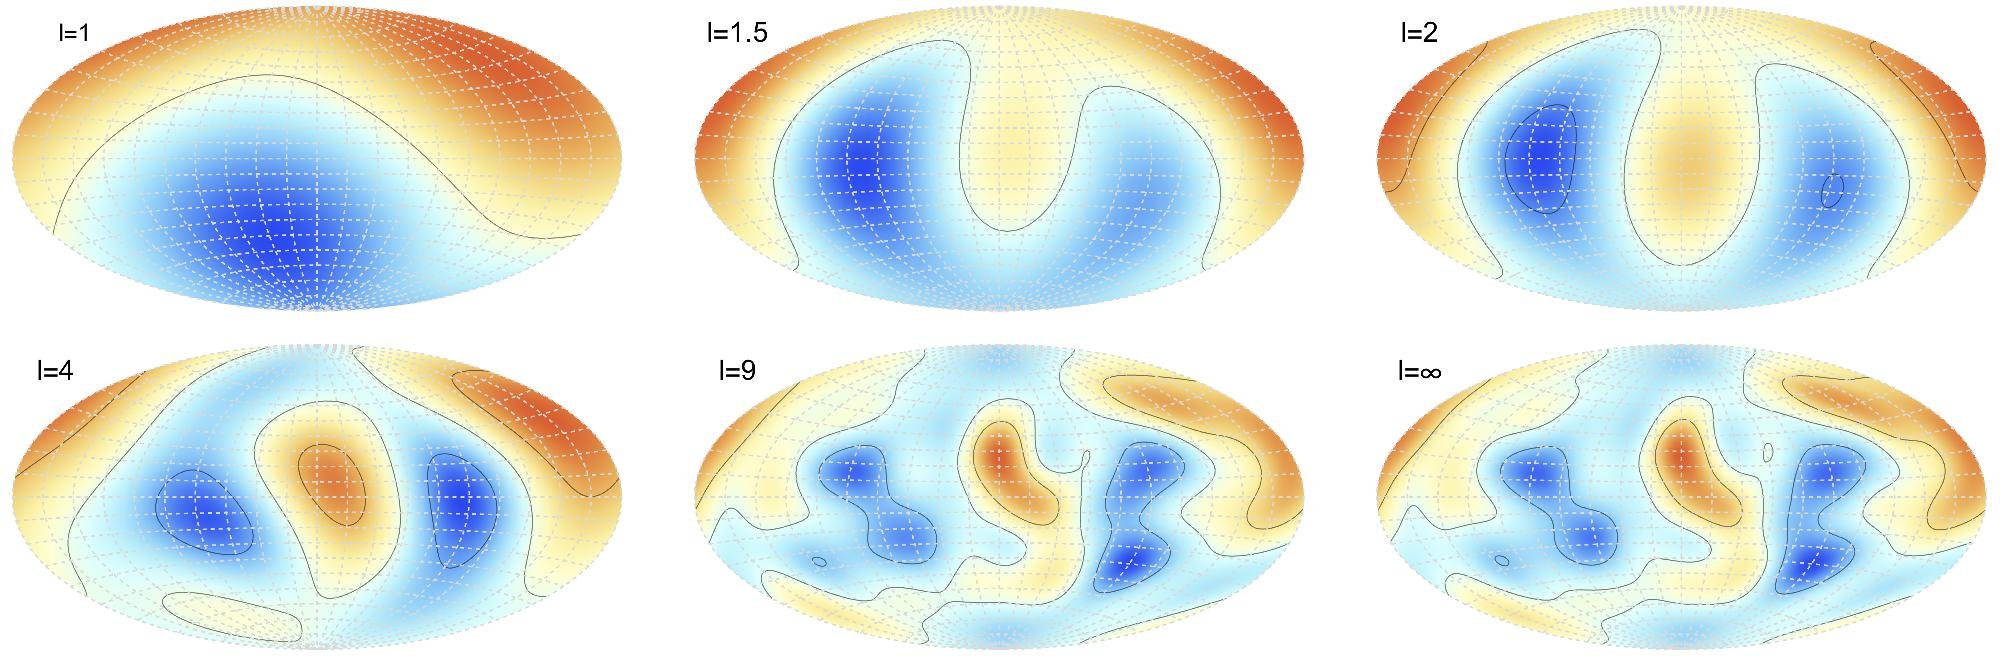
\includegraphics[width=4in]{figures/fig1.pdf}
\caption{\small{a) The local universe interior to the CMB photosphere expressed in comoving coordinates. The circles are, in order, $a=0.6$, ($z\sim0.7$), schematically the limit of present surveys, $a=0.3$, ($z\sim2$) roughly the effective limit of future surveys, the nominal Epoch of Reionization at $a=0.1$, ($z\sim9$ and the CMB photosphere at $a=0.00093$, ($z\sim1100$) and a distance $x=1$. The comoving radius of the big bang is $14.2$~Gpc. Also shown as dashed lines are the nodes of a single wave mode with $k\sim0.45$~Gpc$^{-1}$ which contributes significantly to spherical harmonics with $\ell\leq8$. b) Variation of the amplitude of this wave with scale factor $a$.}}
\end{figure}
\subsection{Fourier Expansion of the Potential}
It is conventional to Fourier expand the potential $\Phi({\bf x}$ today. Although the full spectrum of the Fourier modes we are discussing is continuous in ${\bf k}$ (where $\bf k$ is measure in units of (13.9~Gpc)$^{-1}$, the fact that our observations are made over a restricted volume means that we can treat the waves as a discrete Fourier transform of modes associated with a box in comoving space of side $L$ on which periodic boundary conditions are imposed. If $L$ is too small, the enforced periodic boundary conditions will strongly distort the map; if $L$ is too large, the mode spacing in k-space will be too fine and the modes will not be independent. $L$ is chosen here to have a compromise value of $L=4$, which we discuss further below.
\begin{equation}
\Phi[{\bf x}(r,\theta,\phi)]=\sum_{n=1}^{N/2}[f_n\cos({\bf k}_n\cdot{\bf x})+f_{N+1-n}\sin({\bf k}_n\cdot{\bf x})]
\end{equation}
where the coefficients $f_n$ are real and ${\bf k}=\Delta k{\bf n}=\Delta k\{n_1,n_2,n_3\}=k\{\sin\theta'\cos\phi',\sin\theta'\sin\phi',\cos\theta'\}$, with $n_1,n_2,n_3$ integers and $\Delta k=2\pi/L=\pi/2$.  We restrict the sum to $(n_1^2+n_2^2+n_3^2)^{1/2}\le n_{\rm max}$ and only need consider $\bf k$ over a hemisphere (since the potential must everywhere be real.) We label the coefficients by the index $n$ running from $1$ to $N\sim4\pi n_{\rm max}^3/3$. ($N=6,32,122,256,514,924,1418,2108,3070,4168$ for $n_{\rm max}=1$ through $10$ which will suffice for this paper.)
\subsection{Sachs-Wolfe Limit}
Our input data comprises CMB temperature fluctuations from recombination $\delta(\theta,\phi)\equiv\delta T/T$, where $\theta,\phi$ are spherical polar coordinates measured with respect the same axes as the $\theta',\phi'$ used for $\bf k$. As we are confining attention to long wavelength Fourier components we will only need small $\ell$ spherical harmonics to describe $\delta$. The transverse scales are large compared with the thickness of the photosphere and this implies that the dominant cause of the temperature fluctuation is the gravitational redshift --- the Sachs-Wolfe effect --- that $\Phi=3\delta$, allowing for the expansion in the usual manner. This is increasingly inaccurate for $\ell\gtrsim30$ and we use the more accurate relation between $\delta$ and $\Phi$, though, for this paper the difference is insignificant.
\subsection{Spherical Harmonic Expansion and Response Matrix}
$\delta$ and, consequently, $\Phi({\bf x})$ can be expanded formally as a finite sum of spherical harmonics --- the generalisation of Fourier modes to a sphere --- up to and including the $\ell_{\rm max}$ shell:
\begin{equation}
\Phi=\sum_1^{(\ell_{\rm max}+1)^2}a_yY_y
\end{equation}
where $Y_y$ is a vector of real spherical harmonics:
\begin{equation} 
Y_y(\theta,\phi)=\{Y_{0,0},Y_{1,0},2^{1/2}\Re[Y_{1,1}],2^{1/2}\Im[Y_{1,1}],Y_{2,0},\dots,2^{1/2}\Im[Y_{\ell_{\rm max},\ell_{\rm max}}]\}
\end{equation}
of length $(\ell_{\rm max}+1)^2$ and where $\theta,\phi$ are standard spherical polar coordinates. Note that there are $2\ell+1$ independent, real, basis function in each $\ell$-shell. (The use of a real basis helps identify systematic effects.) Note also that $\int d\Omega Y_yY_{y'}=\delta_{yy'}$. It is convenient to treat $\ell_{\rm max}$ as a continuous variable by adding a fraction between zero and unity of the largest $\ell$ shell and thereby change the angular resolution continuously. 
\begin{figure}[t]
\centering
%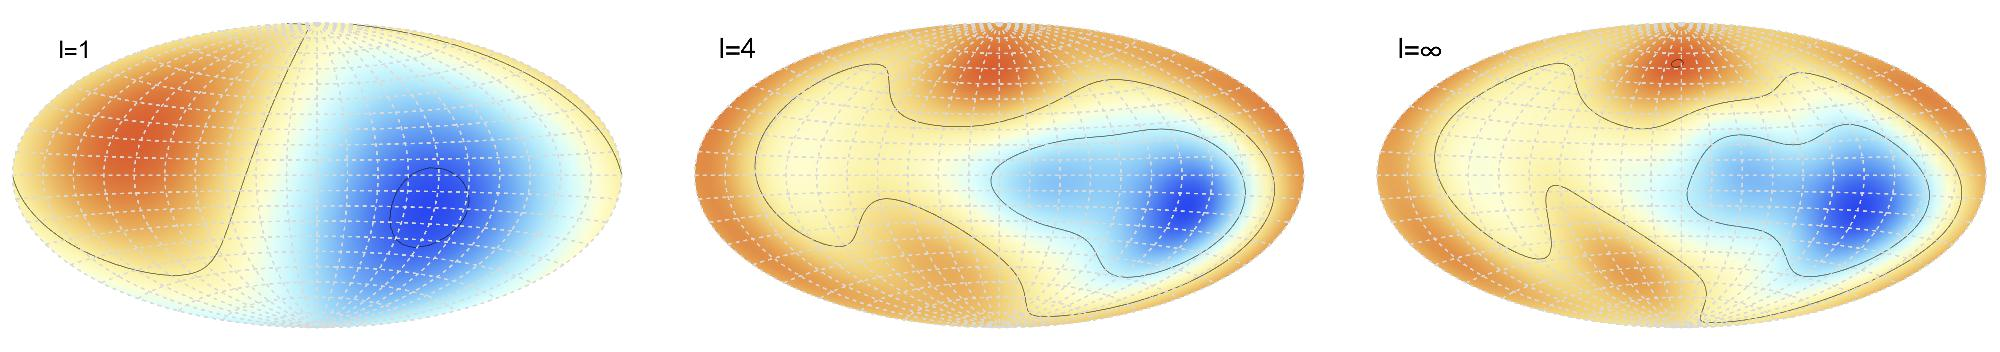
\includegraphics[width=6in]{figures/fig2.jpg}
\caption{{\small Photospheric potential fluctuations of the CMB for $\ell_{\rm max}=2,4.5,10$ (derived from Planck data) and shown as Mollweide projections.}}
\end{figure}

We wish to relate a specific realization of the CMB temperature fluctuations to the underlying Fourier  spectrum. We first expand $\Phi({\bf x})$ as a finite sum of Legendre polynomials:
\begin{equation}
\Phi({\bf x;\ell_{\rm max}})=\sum_{\ell=0} ^{\ell_{\rm max}}(2\ell+1)\sum_{n=1}^{N/2}j_{\ell}(k_nx)P_{\ell}({\hat{\bf k}}_n\cdot{\hat{\bf x}})[\cos(\ell\pi/2)f_n+\sin(\ell\pi/2)f_{N+1-n}].
\label{eqphisum}
\end{equation}
We next introduce the response matrix ${\mathbf R}_{yn}$ which relates individual Fourier coefficients to spherical harmonic coefficients on the recombination sphere $x=1$.
\begin{equation}
a_y={\mathbf R}_{yn}f_n.
\end{equation}
Using Eq.~(\ref{eqphisum}), we find that 
\begin{equation}
\mathbf{R}_{yn}=4\pi Y_y(\theta'\phi')j_\ell(k)[\cos(\pi\ell/2),\sin(\pi\ell/2)]\ {\rm for}\ [1\le n\le N/2,\ N/2<n\le N].
\end{equation}
Typically, the length of $f_n$ will exceed that of $a_y$ and we must find the most likely values of $f_n$ for a given vector $a_y$.
\subsection{Monopole and Dipole Components}
The sums over $y$ include the monopole and dipole terms. These are in a sense unknowable because we do not know the CMB temperature at this time averaged over a volume larger than our horizon and we cannot remove the peculiar motion of the Earth sufficiently carefully to measure the $\ell=1$ coefficients. However, Planck does report these values\dots 
\section{Reconstruction of the Interior Potential}
\subsection{Gaussian Prior}
The ``holographic'' reconstruction that we are attempting has a fundamental limitation in that $O(\ell_{\rm max}^3)$ Fourier components $f_n$ are needed fro $O(\ell_{\rm max}^2)$ spherical harmonic coefficients $a_y$. We need additional constraints. One source of these, important for low resolution reconstruction, comes for highly accurate temperature measurements which imply, in practice, that high order $a_y$ can contribute to low order $f_n$. That this is not sufficient can be seen by considering the problem of inferring the interior temperature of the Earth from very accurate surface measurements alone. We would have no way of distinguishing a solution where the isotherms extended into the core, well spaced from the correct answer where they are bunched up just below the surface. In the present case, the additional information is contained in our hypothesis that the $f_n$ are drawn from a Gaussian distribution with variance satisfying:
\begin{equation}
\sigma_\mathbf{n}^2=\sigma_1^2n^{n_s-4},
\end{equation}
where $n_s$ is measured to be 0.96 (1 suffices for the present purpose) and $\sigma_1^2/2\pi^2L^3\equiv\frac{d<\Phi^2>}{d\ln k}$, the dimensionless variance of a mode with $k=\Delta k$ today is measured to be ???. We reiterate that the spectrum of the power law is derived from a study of the full range of spherical harmonics, $2\le\ell\lesssim5000$ not just from the modes that are actually used in the analysis. We discuss the sensitivity of our maps to the chosen spectrum and the assumption of Gaussianity below.
\subsection{Maximum Likelihood Estimator}
We now explain how to characterize the posterior PDF (which under our assumptions is a multi-variate Gaussian distribution) for each of the coefficients $f_n$ by first finding its peak, minimizing the quantity
\begin{equation}
-2\ln{\cal P}\left(f_n|a_y\right) \approx (a_y- f_n\mathbf{R}_{ny})C_{yy'}^{-1}(a_{y'}-\mathbf{R}_{y'n'}f_{n'})+\frac{f_n^2}{\sigma_{{\bf n}}^2} + \mathrm{const.}
\end{equation}
with respect to variation of $f_n$. Here, $C_{yy'}^{-1}$ is the inverse of the covariance matrix. This leads to the linear equations:
\begin{equation}
f_n=\left(\mathbf{R}_{ny}C_{yy'}^{-1}\mathbf{R}_{y'n'}+\frac{\delta_{nn'}}{\sigma_{\bf n}^2}\right)^{-1}\mathbf{R}_{n'y}C_{yy'}^{-1}a_{y'}
\label{eq:bayes}
\end{equation}
\subsection{Uncertainties}
This is an approach that should produce values for the $f_n$ as long the covariance matrix is well-defined. This does not guarantee that they are meaningful and in order to do this, we must devise a procedure to estimate their significance.
\section{Testing the Method}
\subsection{Recovering a Trial Potential}
Before applying this method to the Planck dataset, we should investigate its performance with trial data. We have created 100 mock datasets with $L=4$, $n_\mathrm{max}=4$ and used these to answer some of the questions we have already raised. For each mock dataset, we assign {\it true} Fourier coefficients $f_\mathrm{n\,true}$ adopting the Gaussian prior and using a random number generator. We next convert these to {\it measured} $f_n$ using the Planck covariance matrix. We then create a CMB map on the recombination sphere and evaluate the spherical harmonic coefficients $a_y$ up to $\ell_\mathrm{max}=8$. The final step is to use our procedure to recover {\it derived} coefficients $f_\mathrm{n\,der}$ which can be compared with the true values. We adopt a crude  figure of merit for each mock map:
\begin{equation}
F=\frac1N\sum_{n=1}^N\left(\frac{f_\mathrm{n\,der}-f_\mathrm{n\,true}}{\sigma_{\mathbf n}}\right)^2.
\end{equation}
In Fig.~ we compare examples of derived maps with different figures of merit with the original true map. We adopt a figure of merit $F=???$ as an acceptable value for a map.
\subsection{Box Size}
As a first step towards optimizing this procedure, we consider the size of the box, $L$. We repeat the process we have just described for larger and smaller values of $L$ to confirm that we have chosen the best value. 
\subsection{Sensitivity to the Cosmological Model}
We can also confirm that our answers are not sensitive to the assumed cosmological model. We have separately changed $\Omega_\Lambda$ and $\Omega_k$ each by  0.05 and we have also consider dark energy models with $w=-0.9$. We find that $F$ hardly changes.
\subsection{Variation with $n_\mathrm{max}$}
We next consider how the figure of merit is improved as we increase the number of Fourier components, i.e. by increasing $n_\mathrm{max}$. The maximum value that can be used clearly depends upon the accuracy of the measurement of individual Fourier components. We find that with the covariance matrix we have adopted, which is based upon the properties of the Planck data, there is no significant improvement in the figure of merit by increasing $n_\mathrm{max}$.Furthermore, if we reduce the variance by as much as a factor 3, we find only a marginal reduction in $F$ when $n_\mathrm{max}$ is increased by one. However, if we increase $\ell_\mathrm{max}$ from 8 to 12 we find that we can improve the accuracy and increase the resolution of the map by increasing $n_\mathrm{max}$ from 10 to 12. We will discuss how to do this with the existing data by using a more complicated estimator in Paper IV.
\section{Application to the Planck Data Set}
\subsection{Description of Dataset}
In our first attempt to create 3D map we take $N_m=100$ individual Planck sky maps and sample them using the HEALPIX algorithm and then create $N_m$ sets of spherical harmonic coefficients which we convert to out basis to derive $N_m$ sets of coefficients $a_y$. We then used this to recreate the mean coefficients $\bar{a}_y$ and the low resolution sky map. We then constructed a covariance matrix for the measurements of $a_y$:
\begin{equation}
C_{yy'}=<(a_y-\bar{a}_y)(a_{y'}-\bar{a}_{y'})>
\end{equation}
where the average is over all the $N_m$ individual maps. All we are doing here is finding linear combinations of the data that are statistically independent. We find that this matrix is robustly invertible for $\ell_\mathrm{max}\le8$ and confine our attention to this straightforward case. be used directly up to $\ell=8$. We construct the eigenvalues and eigenfunctions of the covariance matrix both over all values of $\ell$ and separately with $\ell$ shells. We observe no unusual patterns in these quantities. We were able to improve the stability of the inversion by renormalizing the coefficients within $\ell$ shells but will not pursue this and other strategies here. 
\subsection{Derived Potential Map}
We are now in a position to use Eq.~(\ref{eq:bayes}) to solve for the Fourier coefficients and exhibit the 3D potential map. We also show the ``true'' $\ell_\mathrm{max}=8$ map and the ``derived'' map which has a figure of merit $F=???$.  It can be seen that there there are xxx potential maxima and xxx potential minima within the recombination sphere today We appear to be close to a potential maximum. We can use these maps to create distributions of the current fractional density perturbation (the local underdensity is $\delta\rho/\rho=-???$. In addition we can create low resolution velocity maps use the perturbation equations and find a value ${\mathbf v} =???$ towards ???
\subsection{Velocity and Density Maps}
We can use these maps to create distributions of the current fractional density perturbation. We appear to be close to a potential maximum with $\delta\rho/\rho=-???$. In addition we can create low resolution velocity maps use the perturbation equations and find a value ${\mathbf v} =???$ towards ???. The errors are derived on the basis of the simulations discussed above.
\subsection{The Universe Beyond our Horizon}
Interestingly, it is possible to make statements about the universe beyond our current horizon. This is structure that will become visible in our future. This might seem surprising but it is really a consequence of our Gaussian prior. To see this suppose our prior were that there was a single Fourier mode we could then project as far beyond our horizon as the accuracy with which we could determine the amplitude and phase and direction of this mode would allow. 
\subsection{Influence of Residual Galactic Foreground}
A major concern relating to this approach is that the large scale structure in our maps is seriously contaminated by the removal of the Galactic foreground. It is encouraging that he structure that we find shows little correlation with major features within the Galaxy but additional tests are underway to quantify this uncertainty.
\section{Discussion}
In this paper, we have developed a simple approach to mapping the 3D Newtonian potential within  the last scattering surface at the epoch of recombination. As the perturbations inferred on the scales we are considering remain quite linear, we can use observations from any part of spacetime on our past lightcone to infer the entire variation within our horizon (and slightly beyond) from the time of inflation to the far future. We have deliberately restricted the input data to CMB temperature fluctuations with $0\ell\leq\ell\leq8$ where the covariance matrix is easily computed and have set aside the abundance of data that could improve the map, or may do so in the future, in order to optimize the method and elucidate the viability and limitations of this approach. The results are encouraging but also bring out how hard it will be to connect detailed maps of small volumes of the universe, especially in our neighbourhood, to structure on the largest scale. We intend to discuss these and closely related matters in the next three papers in this series.
\section*{Acknowledgments}
We are especially grateful to Planck team members Ingunn Wehus \& Hans-Kristian Eriksen for their encouragement and help in furnishing 100 samples of the low resolution Planck temperature data to allow us to complete this pilot project. 
\bibliographystyle{apj}
\bibliography{references}
\end{document}

Observations of temperature fluctuations in the CMB measure the 2D
potential $\Phi$ (considered as a linear perturbation to the
Robertson-Walker metric tensor under the Newtonian gauge) on the
sphere of last scattering (where the scale factor $a\sim0.0009$ and
the time is $t\sim380$~kyr). The measurement is quite direct on large
angular scale ($\ell\lesssim30$) in the ``Sachs-Wolfe'' regime; it is
indirect on small angular scales where velocity and density
perturbations are more important, which are linearly related to the
potential perturbation. It is also possible, at least in principle, to
learn about the first and second radial derivatives of this potential
through studying the polarization. This 2D potential is derived from a
3D potential which fills the sphere and extends beyond our horizon.
This potential is derived from one specific realization of an initial
Fourier spectrum of inferred type and statistical properties.  This
paper reports on an investigation of what can be learned, at least in
principle, about the 3D potential at the time of recombination from
the 2D information. Furthermore, any set of Fourier components can be
evolved assuming the now standard ``Flat $\Lambda$ CDM'' cosmology and
connected to the potential information derivable from large surveys
conducted out to modest redshift. What is being discussed here is an
exercise in basic cartography and not in measuring the physical
behavior of the universe at either early or late times. As with many
such exercises the goal is to understand the approximate arrangement
of structure within the observable universe on the largest linear
scales. We shall be more concerned with the topological organization
of this structure than with precise measurement. However, success in
this endeavor ought to improve the investigation of physics questions
through contributing constraining priors to Bayesian inference
studies.

In Sec. 2, we discuss the basic assumptions that we will make in our
idealized versions of the problem. This is followed in Sec. 3 by a
description o fate Fourier representation of the 3D potential and its
relationship to the spherical harmonic decomposition on the last
scattering sphere. The nesting of equipotential contours on the last
scattering photosphere is analyzed in Sec. 4 and this is generalized
to surfaces in 3D in the following section.  The relationship between
the 2D and 3D equipotentials is discussed in Sec.6. In Sec. 7., we
outline a Bayesian approach to calculating the likeliest form of the
3D potential, paying special attention to the criteria which dictate
the effective resolution of the reconstruction and how this may be
improved by adding interior data. Our conclusions are collected in
Sec. 8. A future publication will apply this approach to actual data.

%%%%%%%%%%%%%%%%%%%%%%%%%%%%%%%%%%%%%%%%%%%%%%%%%%%%%%%%%%%%%%%%%%%%%%

\section{Basic Assumptions}

We  work with an idealized problem which we specify as follows:

\begin{itemize}
\item Represent the big bang as a sphere of comoving radius $\sim14.23$~Gpc (adopting a Hubble constant of 68 km s$^{-1}$ Mpc$^{-1}$) and flat $\Lambda$CDM .  The last scattering surface -- the \emph{cosmic photosphere} --  is a sphere with radius $\sim0.29$~Gpc smaller. Recombination occurs over a short but finite interval of time just prior to last scattering. The radius of the cosmic photosphere, 13.94~Gpc, is our unit of length.
\item Ignore the expansion of the universe and just consider the potential as a set of linear normal modes at the time of last scattering. These can be evolved backward and forward in time with confidence. In practice, the potential changes little after recombination although shorter-wavelength modes eventually become nonlinear. (This, too, can be accommodated in principle.)
\item Consider only scalar modes, setting the tensor contribution to zero. If, one day, a significant tensor component is confidently measured, minor modifications to what follows can be included.
\item Hypothesize that the amplitude of each of these modes is drawn from a Gaussian distribution with zero mean, random phase and initial variance roughly proportional to $k^{-3}$ as is consistent with the observations.
\item Ignore modes with wavelength longer than the side of the box, {L}. Their contributions can be approximately incorporated into the lowest Fourier components in a given box as long as we only care about observations within our horizon. This procedure will improve as we enlarge the box. However if the box is too large the spacing of modes in k-space $\Delta k=2\pi/L$ will be too fine and the amplitudes of neighboring modes will be poorly distinguished. A choice $L\sim4$ turns out to be a good compromise. Truncate the spectrum with a sphere of radius $n_{\rm max}\Delta k$; shorter wavelength modes contribute to the error and a Gaussian window function may be preferable.
\end{itemize}

%%%%%%%%%%%%%%%%%%%%%%%%%%%%%%%%%%%%%%%%%%%%%%%%%%%%%%%%%%%%%%%%%%%%%%

\section{Fourier Modes}
We represent the potential $\Phi$ within the box in polar coordinates
as a Fourier series with wave vectors ${\bf k}=\Delta
k\{n_1,n_2,n_3\}$, with $n_1,n_2,n_3$ integers and $\Delta k=2\pi/L$.
As $\Phi$ is real, we only need to assign one real number to each
mode. We approximate Eq.~(1) by a finite sum restricted to
$(n_1^2+n_2^2+n_3^2)^{1/2}\le n_{\rm max}$ and we label the
coefficients $f_{\bf k}$ by the index $n$ running from $1$ to
$N\sim4\pi n_{\rm max}^3/3$. ($N=6,32,122,
256,514,924,1418,2108,3070,4168$ for $n_{\rm max}=1$ through $10$.) It
is simplest to restrict ${\bf k}$ to a hemisphere and to write:
\begin{equation}
\Phi[{\bf x}(x,\theta,\phi)]=\sum_{n=1}^{N/2}[f_n\cos({\bf k}_n\cdot{\bf x})+f_{N+1-n}\sin({\bf k}_n\cdot{\bf x})]
\end{equation}

\begin{figure*}
\centering
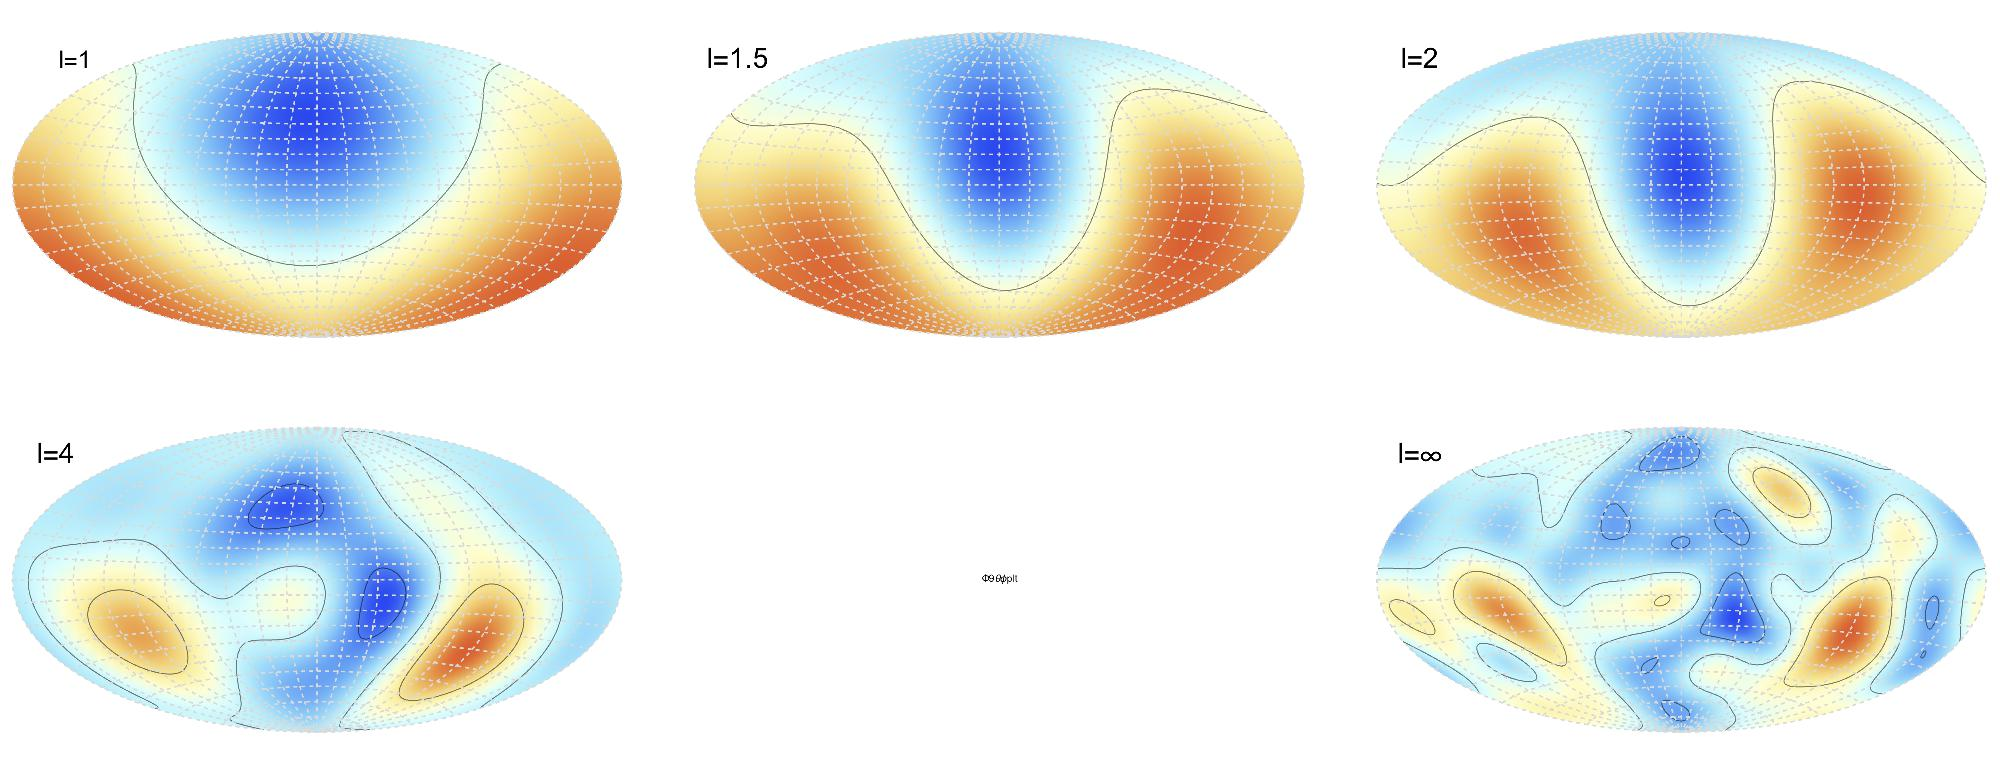
\includegraphics[width=0.9\linewidth]{figures/fig1.jpg}
\caption{Aitoff projections of the potential on the cosmic photosphere $\Phi(\theta,\phi;\ell)$ at $x=1$ for different angular resolutions, parametrized by $\ell$. The contour levels are $0\pm1$. A fixed set of random Fourier components truncated with $n_{max}=3$ is used.}
\end{figure*}

Our main goal is to relate surface information on the photosphere to
the underlying $f_n$.\footnote{This is sometimes called
\emph{holography}, though it is not the original meaning of the word.}
The approach that we will follow is constructive. $\Phi$ can be
expanded exactly as an infinite sum of Legendre polynomials which we
truncate at a finite value of $\ell$, starting with $\ell=1$.

\begin{equation}
\Phi({\bf x;\ell})=\sum_{\ell'=0} ^\ell(2\ell'+1)\sum_{n=1}^Nj_{\ell'}(k_nx)P_{\ell'}({\hat{\bf k}}_n\cdot{\hat{\bf x}}){\cal S}(n,\ell')f_n,
\end{equation}
where ${\bf k}_n={\bf k}_{N+1-n}$ and ${\cal S}(n,\ell)=[\cos(\ell\pi/2),\sin\ell\pi/2)]$, for $[1\le n\le N/2,N/2<n\le N]$. As $\ell$ is increased the effective resolution of $\Phi$, in radius and angle, improves. It is convenient to treat $\ell$ as a continuous variable by the device of summing up to $\lfloor\ell\rfloor$  and then adding the next term in the sum multiplied by $(\ell-\lfloor\ell\rfloor)$. To describe the potential generated by modes with a given value of $n_{\rm max}$, we need spherical harmonics up to $\ell\sim3n_{\rm max}$ and {\it vice versa} (Fig.~1). An immediate implication is that an accurate $\Phi$ map on the sphere, degraded to resolution $\ell$ provides $L=(\ell-1)(\ell+3)$ real numbers which can be used to solve for $N$ real Fourier coefficients suggesting that there is enough information in a $\ell=9$ map to solve for $\sim100$ Fourier components up to $n_{\rm max}\sim3$ independent of the priors on their actual values. When we include the priors, we can proceed to finer scale. Also, when we reduce the radius of the sphere, the value of $n_{\rm max}$  probed by a given $\ell$ scales $\propto x^{-1}$ (Fig. 2).

\begin{figure*}
\centering
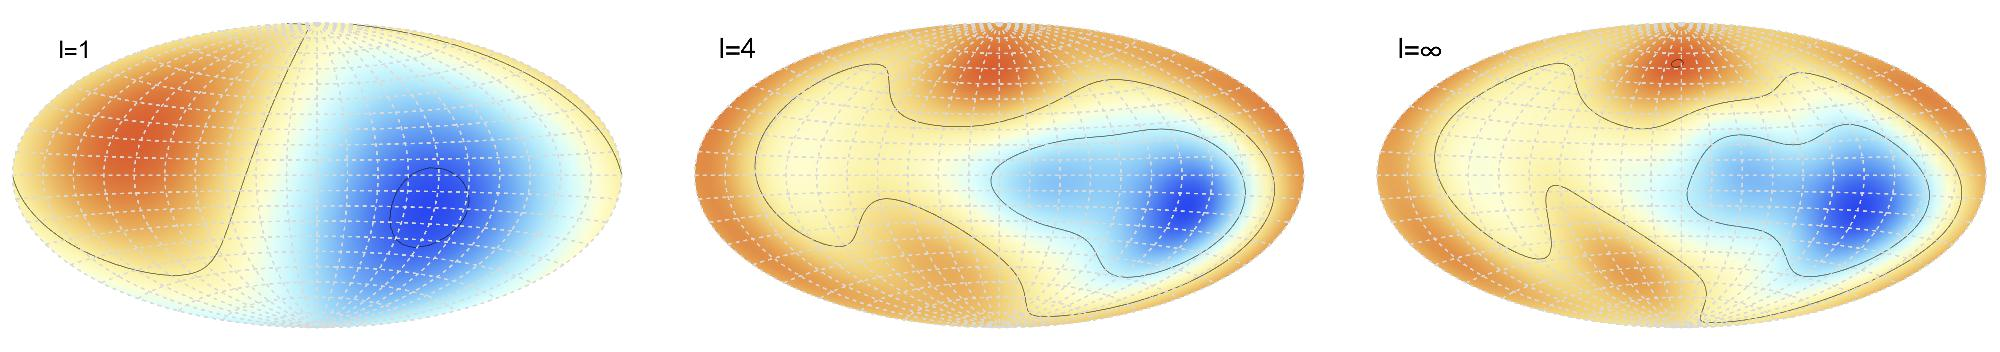
\includegraphics[width=0.9\linewidth]{figures/fig2.jpg}
\caption{Aitoff projections of the potential on a sphere with $x=0.5$ with the same Fourier series as in Fig.~1. The expansion up to $\ell=4$ is a very good approximation to the full potential.}
\end{figure*}


%%%%%%%%%%%%%%%%%%%%%%%%%%%%%%%%%%%%%%%%%%%%%%%%%%%%%%%%%%%%%%%%%%%%%%

\section{Relating Surface and Interior Equipotentials}

Now let us outline how to extract information about the interior
potential from the surface potential. We suppose that we are in the
Sachs-Wolfe region of the spectrum where the surface potential
$\Phi(1,\theta,\phi)=3\delta_T$, where $\delta_T$ is the relative CMB
fluctuation. We set aside for the moment the velocity and density
contributions to the observed fluctuation and the additional
information (roughly twice as much) that can be garnered from adding
polarization maps. We align the 3 axis (Eq.~(1)) with $\theta=0$ and
the 1 axis with $\phi=0$.

Our first task is to describe the inferred potential on the sky. We
suppose this is approximated by a finite sum over spherical harmonics:

\begin{equation}
\Phi(1,\theta,\phi;\ell_{\rm max})=\sum_{y=1}^{(\ell_{\rm max}+1)^2}a_yY_y(\theta,\phi),
\end{equation}
where $Y_y=\{Y_{0,0},Y_{1,0},2^{1/2}\Re[Y_{1,1}],2^{1/2}\Im[Y_{1,1}],Y_{2,0},\dots,2^{1/2}\Im[Y_{\ell_{\rm max},\ell_{\rm max}}]\}$. Note that there are $2\ell+1$ independent, real, basis function in each $\ell$-shell. Note also that $\int d\Omega Y_yY_{y'}=\delta_{yy'}$.

Next, we describe the potential using Eq.~(2) and the identity
\begin{equation}
P_{\ell}[\hat{\bf k}(\theta',\phi')\cdot\hat{\bf x}(\theta,\phi)]=\frac{4\pi}{2\ell+1}\sum_{y=\ell^2+1}^{(\ell+1)^2}Y_y(\theta',\phi')Y_y(\theta,\phi)
\end{equation}
The spherical harmonic coefficients are then given by the linear relation
\begin{equation}
a_y=\Response f_n,
\end{equation}
where we adopt the summation convention and
\begin{equation}
\Response =4\pi i^\ell Y_y^\ast(\theta',\phi')j_\ell(k),
\end{equation}
with $\cos\theta'=n_3/n,\tan\phi'=n_2/n_1$. The elements of the
transformation matrix $\Response$ have been tabulated up to $n_{\rm
max}=6$, $l=10$ which should be sufficient for our purpose.

We estimate the importance of spherical harmonics with order $\ell$ to
the signal at a given given range of $k$ by evaluating the sum:
\begin{equation}
P(\ell;n_{\rm max})=\sum_{n=N(n_{\rm max}-1)+1}^{N(n_{\rm max})}\sum_{y=\ell^2-3}^{(\ell-1)(\ell+2)}|\Response|^2
\end{equation}
\begin{figure}
\centering
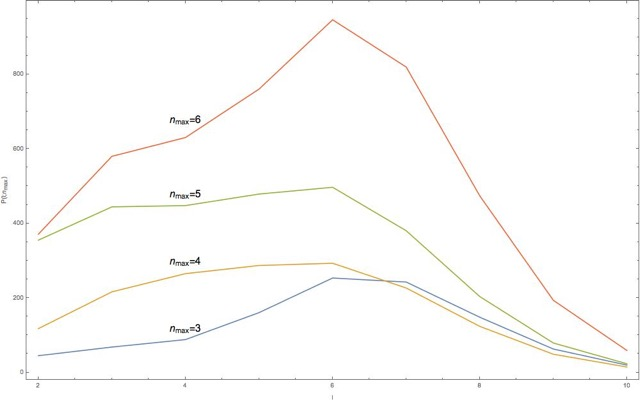
\includegraphics[width=0.9\linewidth]{figures/fig6.jpg}
\caption{Importance of spherical harmonics of order $\ell$ for shells
in k-space with inner radius $n_{\rm max}-1$ and outer radius
$n_{max}$.}
\end{figure}


%%%%%%%%%%%%%%%%%%%%%%%%%%%%%%%%%%%%%%%%%%%%%%%%%%%%%%%%%%%%%%%%%%%%%%

\section{Inferring the 3D Potential}

Our task is to take a given vector of measured spherical harmonic
coefficients $\mathbf{a}$, with covariance matrix $C$,  and
infer a vector of the Fourier coefficients of our model potential,
$\mathbf{f}$,  under the prior assumption that the  components $f_n$
are independent and drawn from a Gaussian distribution with variance
$\sigma_n^2 = (n_1^2+n_2^2+n_3^2)^{-3/2} / \alpha$. We seek the
posterior PDF ${\cal P} = \Pr(\mathbf{f}|\mathbf{a},\alpha)$, where
\begin{equation}
% -\ln{\cal P} = \frac{(a_y^2-\Response f_n)^2}{2\sigma_y^2}+\frac{f_n^2}{2\sigma_n^2} + \text{const.}
-\ln{\cal P} = (\mathbf{a}-\ResponseMatrix\mathbf{f})^{\rm T} C^{-1} (\mathbf{a}-\ResponseMatrix\mathbf{f})
             + \mathbf{f}^{\rm T} S^{-1} \mathbf{f} + \text{const.}
\end{equation}
and the matrix $S$ is diagonal, with
elements~$S_{nn} = \sigma_n^2$.
Differentiating this expression leads to a set of linear equations
% \begin{equation}
% \left(\frac{\Response m_{yn'}}{\sigma_y^2}+\frac{\delta_{nn'}}{\sigma_n^2}\right)f_{n'}=\frac{a_y\Response}{\sigma_y^2},
% \end{equation}
which can be solved for the maximum posterior 3D potential
Fourier coefficients $\mathbf{f}_{\rm MP}$, given a choice of power spectrum
normalisation~$\alpha$. We follow \citep{SuyuEtal2006} and infer the
most probable normalisation~$\alpha_{\rm MP}$ using the Bayesian Evidence,
which leads to the approximate condition
\begin{equation}
    (\mathbf{a}-\ResponseMatrix\mathbf{f}_{\rm MP})^{\rm T} C^{-1} (\mathbf{a}-\ResponseMatrix\mathbf{f}_{\rm MP})
                 + \mathbf{f}_{\rm MP}^{\rm T} S^{-1}(\alpha) \mathbf{f}_{\rm MP} \approx N/2
\end{equation}
where $N$ is the number of spherical harmonic coefficients used. An
iterative scheme was used to optimize $\alpha$ in this way.

We note that the covariance matrix of the measured spherical harmonic
coefficients should not include any cosmic variance terms, because we
are interested in inferring the 3D potential in our one observable
universe. To estimate this object, we took 100 posterior sample
``Commander-Ruler'' temperature maps, decomposed each of them into
spherical harmonics,\footnote{We use the {\sc healpy} code provided at
\texttt{https://healpy.readthedocs.org}.} and then calculated the
sample variance and sample covariance of the coefficients.

\section{Introduction}
\ni{\bf Mapping Our Universe:}
The earliest examples of astronomy included following the nearby planets and charting the ``fixed'' stars which were projected onto the celestial sphere and organized into constellations. Ultimately this led to a physics-based, low resolution,  3D description of the Galaxy. The situation today in cosmology is somewhat similar. We have large surveys of comparatively nearby galaxies~\cite{Kaiser2002, Ivezc2002, Davis2003, Giavalisco2004, DES2005, %Frith:2005az, Frith2005
Skrutskie2006, Faber2007, Scoville2007, Kaiser2010, Blake2011, Alam2015} and a splendid two dimensional map of the microwave background~\cite{Planck2015maps} and this has led to a standard model of the universe in which inflation-based, Gaussian, potential fluctuations, with a well-defined spectrum, grew according to deterministic laws to produce contemporary large scale structure in a flat universe endowed with a cosmological constant. However, the traditional goal of astronomy, to describe the complete disposition of this actual structure, has hitherto been subsumed into statistical investigations designed to elucidate the underlying physics.

This is a staged proposal to combine recent observations with what we have learned about the physics to make the best map we can of the 3D structure of the universe within and slightly beyond our horizon. In addition to satisfying a natural desire to describe our universe, success in this program will naturally furnish ongoing and planned physics investigations with additional priors which should tighten up their accuracy.

\ni{\bf Contents:}
The last decade has seen remarkable advances in cosmology, spearheaded by increasingly detailed measurements of the cosmic microwave background (CMB) radiation~(see e.g.\ \cite{Planck2015maps,Planck2015cosmopara}).
% SPT?, ACT?}.
These accurate measurements have affirmed that a description of a homogeneous, spatially flat general relativistic universe with relatively few ingredients -- photons ($T_\gamma=2.7$~K), neutrinos (three flavors), baryons ($\Omega_b=0.05$), dark matter ($\Omega_d=0.26$) and a cosmological constant ($\Omega_\Lambda=0.69$) supplemented by (almost) scale-free, adiabatic, Gaussian initial perturbations suffices to describe essentially all that is secure in the observations~\cite{Planck2015cosmopara}. There is still room for revision, retraction and major discovery but, right now, we have a good working hypothesis that the universe is basically this simple (e.g.~\cite{Weinberg2008, Schneider2015}). There is some tension in the reported measurements, \eg of the Hubble constant, but this is not important for our purpose and we shall simply adopt Planck values. Much effort is being expended to see if a ubiquitous and eternal cosmological constant needs to be replaced by a dynamical dark energy. If this turns out to be true then simple changes will be needed to what follows.

\ni{\bf Evolution:}
The description of the average expansion of the universe is relatively uncontroversial. When  $t\sim 50$~kyr,  the scale factor -- the size of a region relative to its contemporary size -- was $a\sim0.0003$ and the universe became (dark) matter-dominated. When $t\sim380$~kyr, $a=0.00093$, the hydrogen plasma quickly formed atoms, decoupling from the radiation and forming the inside-out, CMB photosphere where the majority of CMB photons we observe today were last scattered with a temperature $\sim2900$~K. When $t\sim600$~Myr, $a\sim0.1$, the first stars formed and the universe (re)-ionized. This epoch is becoming accessible to observation. Finally when $t\sim8$~Gyr, $a\sim0.6$, the cosmological constant began to dominate the matter, and the universal expansion started to accelerate.

\ni{\bf Fluctuations:}
The observed fluctuations are adequately described by a set of spatial Fourier modes expressed in terms of contemporary or comoving coordinates. These modes are longitudinal and the ones that mostly concern us here evolved linearly. It is convenient to describe their amplitude using the (effective) Newtonian potential/gauge $\Phi$ from which the density and fluid velocity perturbations can be computed (in the ``Sachs-Wolfe'' limit at long wavelength~\cite{Sachs1967}). \footnote{There may also be tensor modes which we shall ignore here. If, and when, they are detected, only minor modifications will be needed.} The modes that mostly concern us remain linear and are ``adiabatic'', so that we only need to know their amplitude and phase at one epoch, e.g. recombination, to predict them for all time.

It has recently been demonstrated, mainly using CMB observations~\cite{Planck2015cosmopara}, that the adiabatic hypothesis is quite accurate. Furthermore, the amplitudes associated with each mode of the initial potential scale approximately as $k^{-3/2}$ and are drawn from a Gaussian distribution, so that the potential fluctuations associated with each length scale are scale-independent. This behavior is consistent with a remarkable early conjecture by Harrison~\cite{Harrison1970} as elaborated by Zel'dovich~\cite{Zeldovich1972}.

The potential associated with a mode was essentially frozen until it ``entered the horizon,'' that is, until the timescale for its dynamical evolution, became smaller than the expansion timescale. We are mostly concerned with long wavelength modes for which this happened after recombination and $k\lo40{\rm Gpc}^{-1}$.\footnote{$k_0$ can be considered as approximately the wavenumber associated with the first acoustic peak and its consequence, Baryon Acoustic Oscillations (BAO).} For such wavenumbers, the waves evolve at roughly constant $\Phi$ until the cosmological constant takes over and the potential falls by roughly 20 percent today. We make this explicit in Fig.~1 where we show the interior of the last scattering surface in comoving coordinate space and a particular wave whose amplitude and phase we are trying to measure.
\begin{figure}[t]
\centering
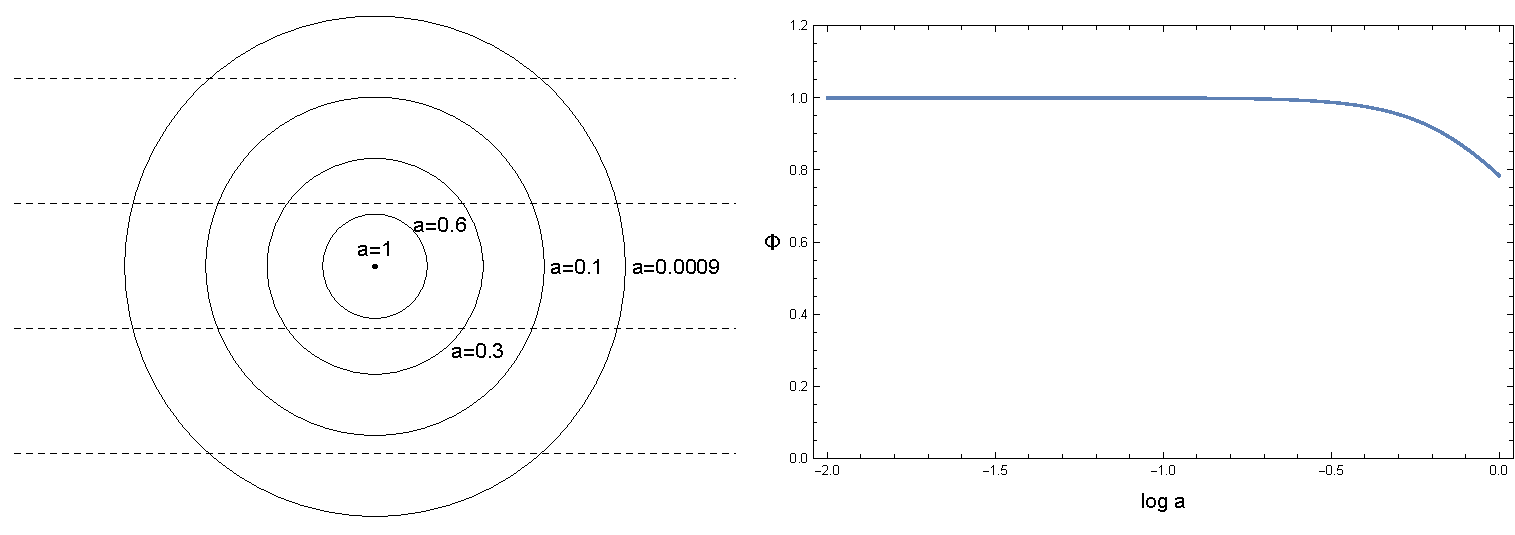
\includegraphics[width=4in]{figures/nsffig1.pdf}
\caption{\small{a) The local universe interior to the CMB photosphere expressed in comoving coordinates. The circles are, in order, $a=0.6$, ($z\sim0.7$), schematically the limit of present surveys, $a=0.3$, ($z\sim2$) roughly the effective limit of future surveys, the nominal Epoch of Reionization at $a=0.1$, ($z\sim9$ and the CMB photosphere at $a=0.00093$, ($z\sim1100$) and a distance $x_{\rm CMB}\sim13.9$~Gpc. The comoving radius of the big bang is $14.2$~Gpc. Also shown as dashed lines are the nodes of a single wave mode with $k\sim0.45$~Gpc$^{-1}$ which contributes significantly to spherical harmonics with $\ell\lo10$. b) Variation of the amplitude of this wave with scale factor $a$.}}
\end{figure}

\ni{\bf Inflation:}
The flatness of the geometry today, the isotropy of the CMB temperature, and the very existence of fluctuations with wavelengths longer than naively allowed by causality are all consistent with the simplest version of a much more specific and even bolder conjecture by Guth~\cite{Guth1981}, Linde~\cite{Linde1982a} and others (e.g.~\cite{%Press1980,
 Mukhanov:1981xt, Sato1981, Hawking1982, Starobinsky1982, Albrecht1982, %Linde1982b, Abbott1982, Guth1982,
  Bardeen1983%, Linde1983, Turner1983, Brandenberger1983, Moss1985, Sasaki1986, Mukhanov1988
  }), that the universe underwent a period of ``inflation'' at much earlier times. This theory is based on the idea that all the structures in the observed universe emerged from quantum fluctuations about $10^{-33}$ seconds after the Big Bang. Inflation, which describes a phase of accelerated cosmic expansion, is the leading theory providing a causal mechanism for generating these fluctuations and stretching them to cosmological scales%(as first realized in~\cite{Mukhanov:1982nu,  %Brandenberger1984, Linde1986a, Linde1986b, Linde1993 Mukhanov1985, })
. The microphysics of inflation makes detailed predictions for the spectra of these fluctuations as observed in the CMB, in particular a slight tilt in the power spectrum, which has been measured (see e.g.~\cite{Malik2008, Gordon2000} and references therein).

%This paragraph is facultative:
Qualitatively, the causal mechanism seeding the primordial perturbations is easily understood. During inflation, the Hubble radius, $H^{-1}$, which can be thought of as the ``apparent horizon", was roughly constant. Meanwhile, quantum fluctuations in the matter field(s) and metric are constantly generated with wavelength $H ^{-1}$ at most~\cite{BirrellsBook1984}. Once produced, a fluctuation with comoving wavelength $\lambda$ is stretched with the expansion of space past the Hubble radius, at which point its dynamical timescale, $\sim ac/k$ was larger than the expansion time and it ``exited'' the horizon and its amplitude froze.  Throughout inflation, such fluctuations are continuously created at the physical scale $H^{-1}$. Therefore, by the end of inflation, perturbations will finally have been produced on a whole spectrum of physical scales.


% therory of cosmological perturbations: Lifshitz1946, Lifshitz1963, Bardeen:1980


\section{Proposed Research}
The long term goal of this proposal is to connect the CMB to local surveys, and to produce an evolving three-dimensional (or in other words, a 4D) map of the universe that is valid from before 380~kyr to today, and out beyond 14 Gpc. The exercise is not purely cartographic as it is essential that we use the secure physical inferences that have been drawn about the early universe in making this map.

The first stage of our proposed program uses 2D CMB observations alone to test internal consistency and to recover as much as we can of the 3D potential, velocity and density fields interior to the last scattering surface. In the second stage, we augment CMB data with existing 3D measurements from galaxy surveys, gravitational lensing, intermediate Sachs-Wolfe measurements and so on. This should improve the resolution. The third stage involves estimating the improvement that should come on a decade timescale from future surveys such as LSST and Epoch of Reionization investigations, ``Stage IV'' CMB observations, SKA etc. The fourth and final stage is an investigation of how far it is possible, even in principle,  to reconstruct the structure of the universe including what can be inferred beyond our horizon.

% - - - - - - - - - - - - - - - - - - - - - - - - - - - - - - - - - -

\subsection{Stage 1. From 2D to 3D: Potential Reconstruction from CMB Data}
\ni{\bf Temperature Fluctuations:}
Most quantitative cosmology derives from CMB observations. The conventional way to describe the observations is in terms of spherical harmonics -- the generalization of Fourier modes to a sphere -- labeled by $\ell$ and $m$. It is convenient to use an equivalent vector of real spherical harmonics, $Y_y(\theta,\phi)=\{Y_{0,0},Y_{1,0},2^{1/2}\Re[Y_{1,1}],2^{1/2}\Im[Y_{1,1}],Y_{2,0},\dots,2^{1/2}\Im[Y_{\ell_{\rm max},\ell_{\rm max}}]\}$ of length $(\ell_{\rm max}+1)^2$ and where $\theta,\phi$ are standard spherical polar coordinates. Note that there are $2\ell+1$ independent, real, basis function in each $\ell$-shell. Note also that $\int d\Omega Y_yY_{y'}=\delta_{yy'}$. It is convenient to treat $\ell_{\rm max}$ as a continuous variable by adding a fraction between zero and unity of the largest $\ell$ shell and therefore smoothly change the angular resolution. (The use of a real basis helps identify systematic effects.)
\begin{figure}[t]
\centering
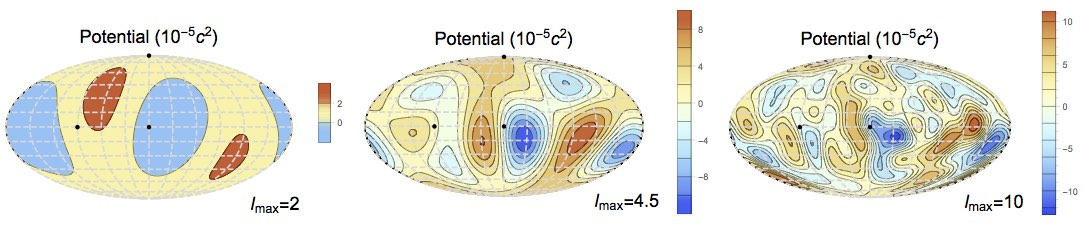
\includegraphics[width=6in]{figures/nsffig2.jpg}
\caption{{\small Photospheric potential fluctuations of the CMB for $\ell_{\rm max}=2,4.5,10$ derived from Planck data shown as Mollweide projections.}}
\end{figure}

Most investigations have focused on measuring the ``power'' in the temperature fluctuations (including polarization) associated with a given $\ell$, obtained by summing products of the coefficients of the harmonic components over $m$, and comparing it with the predictions of various cosmological models. This program has been wonderfully productive, and has resulted in the world model just outlined. Furthermore this power spectrum has been successfully reconciled with features of the local universe, such as galaxy counts. One common assumption is that the particular realization of the universe that we are observing is drawn from a statistical ensemble of universes. When $\ell$ is large, we have many independent measurements on the associated angular scale, $\sim\pi/\ell$, and so we can measure an rms value for the harmonic component with a small variance. However, when $\ell$ is small, we have only a few such measurements and the ``cosmic'' variance is large. Despite their great value, these statistical measurements inevitably discard information which may be valuable.\footnote{This is in the sense that music is far more than a ``flicker'' power spectrum. To pursue our musical metaphor, different voices and instruments contribute different ranges of frequencies to a musical performance over a total range of roughly ten octaves. We are only listening to the bass range but higher voices and instruments can still contribute to what we hear.}  In the proposed study, only one specific realization of the universe -- the one we inhabit --  is considered.

In order to start us on a pilot investigation, Planck team members Wehus \& Eriksen  (Oslo) have kindly supplied 100 sample Planck temperature fluctuation maps for $0\le\ell\le10$ or $1\le y\le121$. From this ensemble we are able to compute the mean photospheric potential fluctuation map at the time of recombination $\Phi=a_yY_y$, (including the monopole and dipole components and adopting the summation convention) and the covariance matrix $C_{yy'}$ associated with the harmonic components $a_y$. We find that this matrix is invertible and can be used directly up to $\ell=8$. More careful treatment of the data is needed beyond this. The fractional variance in individual harmonics varies between $\sim0.0001$ and $\sim0.01$. Undoubtedly, there are systematic effects present in this data set which need to be explored, but the accuracy is high enough to proceed without this.

\ni{{\bf Fourier Modes:}
It is conventional to Fourier expand the potential $\Phi$ today; the expansion at other times is then simply calculable. Although the full spectrum of the Fourier modes we are discussing is continuous in ${\bf k}$, the fact that our observations are made over a restricted volume means that we can treat the waves as a discrete Fourier transform of modes associated with a box in comoving space of side $L$ on which periodic boundary conditions are imposed. $L$ is chosen here to have a compromise value of four times the radius of the CMB photosphere, $13.9$~Gpc which we adopt as our unit of length.
\begin{equation}
\Phi[{\bf x}(r,\theta,\phi)]=\sum_{n=1}^{N/2}[f_n\cos({\bf k}_n\cdot{\bf x})+f_{N+1-n}\sin({\bf k}_n\cdot{\bf x})]
\end{equation}
where the coefficients $f_n$ are also real and ${\bf k}=\Delta k\{n_1,n_2,n_3\}=k\{\sin\theta'\cos\phi',\sin\theta'\sin\phi',\cos\theta'\}$, with $n_1,n_2,n_3$ integers and $\Delta k=2\pi/L=\pi/2$.  We restrict the sum to $(n_1^2+n_2^2+n_3^2)^{1/2}\le n_{\rm max}$ and only need consider $\bf k$ over a hemisphere (since the potential must everywhere be real.) We label the coefficients by the index $n$ running from $1$ to $N\sim4\pi n_{\rm max}^3/3$. ($N=6$ through $4168$ for $n_{\rm max}=1$ through $10$.) $\Phi({\bf x})$ can be expanded formally as an infinite sum of Legendre polynomials and approximately as a finite sum:
\begin{equation}
\Phi({\bf x;\ell_{\rm max}})=\sum_{\ell=0} ^{\ell_{\rm max}}(2\ell+1)\sum_{n=1}^{N/2}j_{\ell}(k_nx)P_{\ell}({\hat{\bf k}}_n\cdot{\hat{\bf x}})[\cos(\ell\pi/2)f_n+\sin(\ell\pi/2)f_{N+1-n}].
\end{equation}

\ni{\bf Gaussian Prior:}
Detailed study of the CMB (e.g.~\cite{Aghanim:2015xee, Ade:2015ava}) has led to the conclusion that the amplitude of each discrete mode with wave vector $\bf k$ is well modeled as having been drawn from a Gaussian distribution of variance $\sigma_{\bf n}^2=\alpha^2(n_1^2+n_2^2+n_3^2)^{-3/2}$. Adopting this model, we can determine the coefficient $\alpha$ approximately and empirically, by computing the spherical harmonic coefficients $a_y =\mathbf{R}_{yn}f_n$ for sets of Gaussian $f_n$s where the ``response matrix'' is given by:
\begin{equation}
\mathbf{R}_{yn}=4\pi Y_y(\theta'\phi')j_\ell(k)[\cos(\pi\ell/2),\sin(\pi\ell/2)]\ {\rm for}\ [1\le n\le N/2,\ N/2<n\le N]\, ,
\end{equation}
and then adjusting $\alpha$ such that the model-predicted and measured spherical harmonics match. This approach is adequate for our pilot study; an improved determination will be investigated following the evidence analysis of~\cite{Suyu2006}, {\sl en route} to a hierarchical modeling of the system where the normalization $\alpha$ is one of a set of hyperparameters governing the statistics of the potential field.

\ni{\bf Preliminary Results:}
The simple question that motivated this investigation, and which did not seem to have a well-known answer, was how much of the 3D potential could be reconstructed interior to the 2D CMB photosphere using CMB observations alone. This is an example of what is sometimes called {\it holography.} At first sight this might seem hopeless, because if one associates $\ell_{\rm max}$ with $k\,x_{\rm CMB}$, then we are trying to solve for $O((k_{\rm max}\,x_{\rm CMB})^3)$ Fourier modes using only $O(\ell_{max}^2)$ spherical harmonics. However, if we confine our attention to the longest wavelength waves,\footnote{Our approach is quite complementary to that of Yadav and Wandelt~\cite{Yadav:2005} who are concerned with wavelengths comparable with the thickness of the recombination surface around the acoustic peak near $\ell\sim200$.} and use all the information that is at our disposal to exploit the high accuracy of the measurements while accepting uncertainty in the result, then it is possible to make some progress.

We approximately characterize the posterior PDF (which under our assumptions is a multi-variate Gaussian distribution) for the coefficients $f_n$ by first finding its peak, minimizing the quantity
\begin{equation}
-2\ln{\cal P}\left(f_n|a_y\right) \approx (a_y- f_n\mathbf{R}_{ny})C_{yy'}^{-1}(a_{y'}-\mathbf{R}_{y'n'}f_{n'})+\frac{f_n^2}{\sigma_{{\bf n}}^2} + \mathrm{const.}
\end{equation}
with respect to variation of $f_n$. Note that $\sigma_{\bf n}$ contains the normalization $\alpha$.

Here, $C_{yy'}^{-1}$ is the inverse
of the covariance matrix. This leads to the linear equations:
\begin{equation}
f_n=\left(\mathbf{R}_{ny}C_{yy'}^{-1}\mathbf{R}_{y'n'}+\frac{\delta_{nn'}}{\sigma_{\bf n}^2}\right)^{-1}\mathbf{R}_{n'y}C_{yy'}^{-1}a_{y'}
\end{equation}

%In Section~\ref{} below, we give a more rigorously-derived expression for the posterior PDF ${\cal P}$.
The approximate form given here is sufficient for a feasibility check:
using mock data, we have found that {\it it is possible to solve for
stable, low order maximum posterior Fourier coefficients, which can
recover harmonic coefficients $a_y$ that are consistent with the
original data.} We have applied this approximate procedure to the
actual Planck data, and our results are exhibited in Fig.~3. There are
features of the data which we have yet to understand but this suffices
to illustrate what we hope will be possible. It is proposed to refine
and improve upon this basic approach to obtain the best map we can
based upon the CMB data alone. In particular we intend to set clear,
statistical criteria for assessing when it is significant to add
additional Fourier components to the map.
%%%%%%%%%%%%%%%%%%%%%%%%%%%%%%%%%
\begin{figure}[t]
\centering
<<<<<<< HEAD
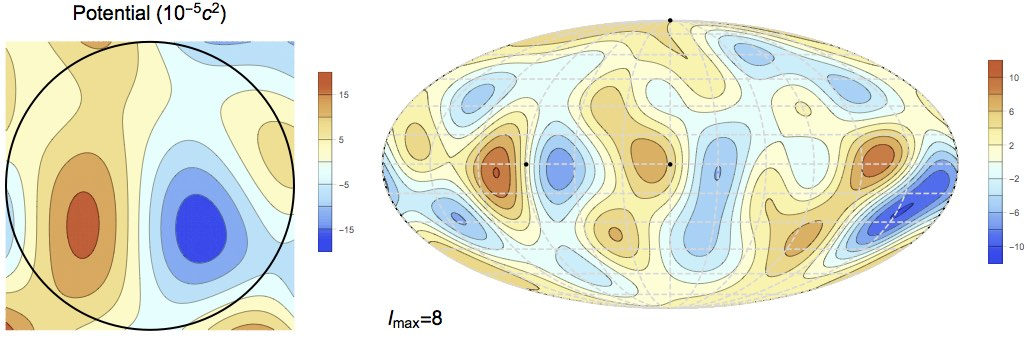
\includegraphics[width=2in]{figures/nsffig3.pdf}
\caption{{\small Figure 3 a) 3D gravitational potential at the time of recombination recovered from 2D fluctuations on the CMB photosphere, which is represented by a circle, and displayed in the $x_3=0$ plane. In this pilot study, 81 spherical harmonics and a Gaussian prior were used to recover 122 Fourier components with $n_{\rm max}=3$. The monopole and dipole were not removed.   b) The potential fluctuations on the CMB photosphere were then recomputed, exhibiting encouraging consistency with the input data.}}
=======
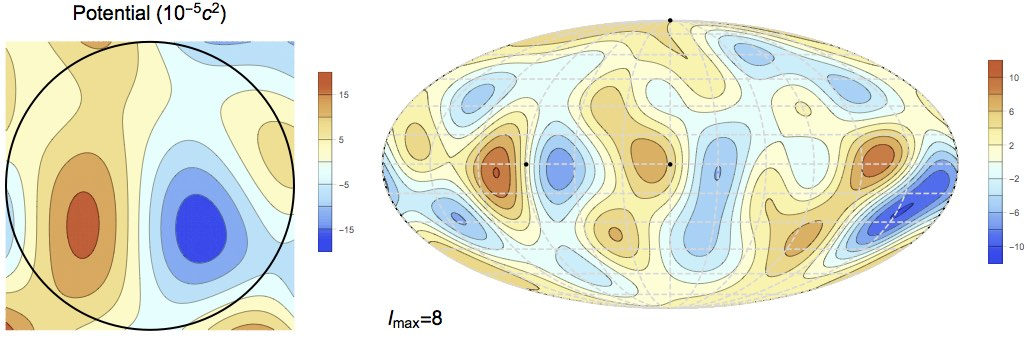
\includegraphics[width=0.9\linewidth]{figures/nsffig3.jpg}
\caption{{\small a) 3D gravitational potential at the time
of recombination, recovered from 2D fluctuations on the CMB
photosphere (represented by the circle), and displayed in the
$x_3=0$ plane. In this pilot study, 81 spherical harmonics and a
Gaussian prior were used to recover 122 Fourier components with
$n_{\rm max}=3$. The monopole and dipole were not removed.   b) The
predicted 2D potential fluctuations on the CMB photosphere
were then recomputed,
exhibiting encouraging consistency with the input data.}}
>>>>>>> fff6f93c75898ae29f1264f24b6e5b58f9faaf30
\end{figure}
%%%%%%%%%%%%%%%%%%%%%%%%%%%%%%%%%

\ni{\bf Inflationary Origin of Perturbations and Hyperparameter Estimation:}
As explained above, inflation provides a mechanism for seeding perturbations in the CMB from quantum fluctuations in the early Universe. It is standard, as we shall do here, for most models to assume that the main matter components during inflation are in the form of scalar fields.%, an assumption which shall be adopted in what follows
Moreover, for simplicity, we shall assume that only one scalar field is dynamically relevant, so that we will work within the framework of ``single-field'' inflation. Apart from these caveats, the framework developed in what follows will remain model-independent.

We want to describe perturbations of the scalar field, which we call $\varphi$, about a homogeneous background. It is common to quantify these perturbations with the gauge-invariant curvature perturbation, $\zeta$.\footnote{At late times (i.e. after the time of BBN) and inside of the horizon, when we use the Newtonian gauge to describe the Newtonian potential $\Phi$, one can think of $\zeta$ and $\Phi$ interchangably. The main advantage of using $\zeta$ during inflation is that, in single-field inflation, the amplitude of its Fourier modes remain constant from horizon exit to horizon re-entry, significantly simplifying their evaluation~\cite{Weinberg2008}.}
%which is defined by:
%\be
%	-\zeta=\psi+H\frac{\delta\rho}{\rho}\, ,
%\ee
%where $\psi$ is the trace part of the spatial scalar metric perturbations, i.e. writing the most general spatial scalar perturbation to a 4-d metric by $\delta g_{ij}=2(\psi\delta_{ij}-E_{ij})$ with $\nabla^2E=0$, then $\psi$ contains the trace of the perturbation. We also define $\rho$ and $\delta \rho$ to be the mean energy density and the linear energy density perturbation, respectively, as well as the $H$, the Hubble parameter.
 In the co-moving gauge, the Fourier modes of $\zeta$ as they exit the horizon are
\be
	\zeta_{{\bf k}}=\sqrt{\frac{\pi}{2}}e^{i\theta}e^{i\frac{\pi}{2}\left(\nu+\frac{1}{2}\right)}(-\tau)^{\nu}\mathcal{H}^{(1)}_\nu(-k\tau)\, .
\ee
Here, $\nu$ is a slowly varying function which encapsulates the specific dynamics of the inflationary model, $\mathcal{H}^{(1)}_\nu$ is a Hankel function of the first kind, $\tau$ is the conformal time, defined by $d\tau=a(t)dt$, and $\theta$ is a random variable endowing each mode with a random phase. A prediction of inflation is that $\theta$ should have a uniform probability distribution between 0 and $2\pi$. This is a fundamental prediction of inflation which stems from the assumption that the fluctuations are quantum mechanical in origin, the very assumption the idea of inflation is based upon.

However, the actual distribution of the phases for the modes of $\zeta$ (or $\Phi$) in the CMB has yet to be measured. This is because, so far, most experiments have strived to measure the power spectrum of fluctuations, $\Delta_\zeta^2$. %defined by:
%\be
%	\Delta_\zeta^2=\frac{k^3}{2\pi^2}\mathcal{P}_\zeta \propto |\zeta_{\vec{k}}|^2\,.
%\ee
Because the power spectrum is proportional to $ |\zeta_{{\bf k}}|^2$, when such a measurement is made, the phase information of the modes is lost. With the reconstruction method proposed in this proposal, such measurement will become possible.

\begin{figure*}[t]
\vspace{-2cm}
\begin{center}
\centering
\begin{minipage}[t]{0.48\linewidth}
\centering
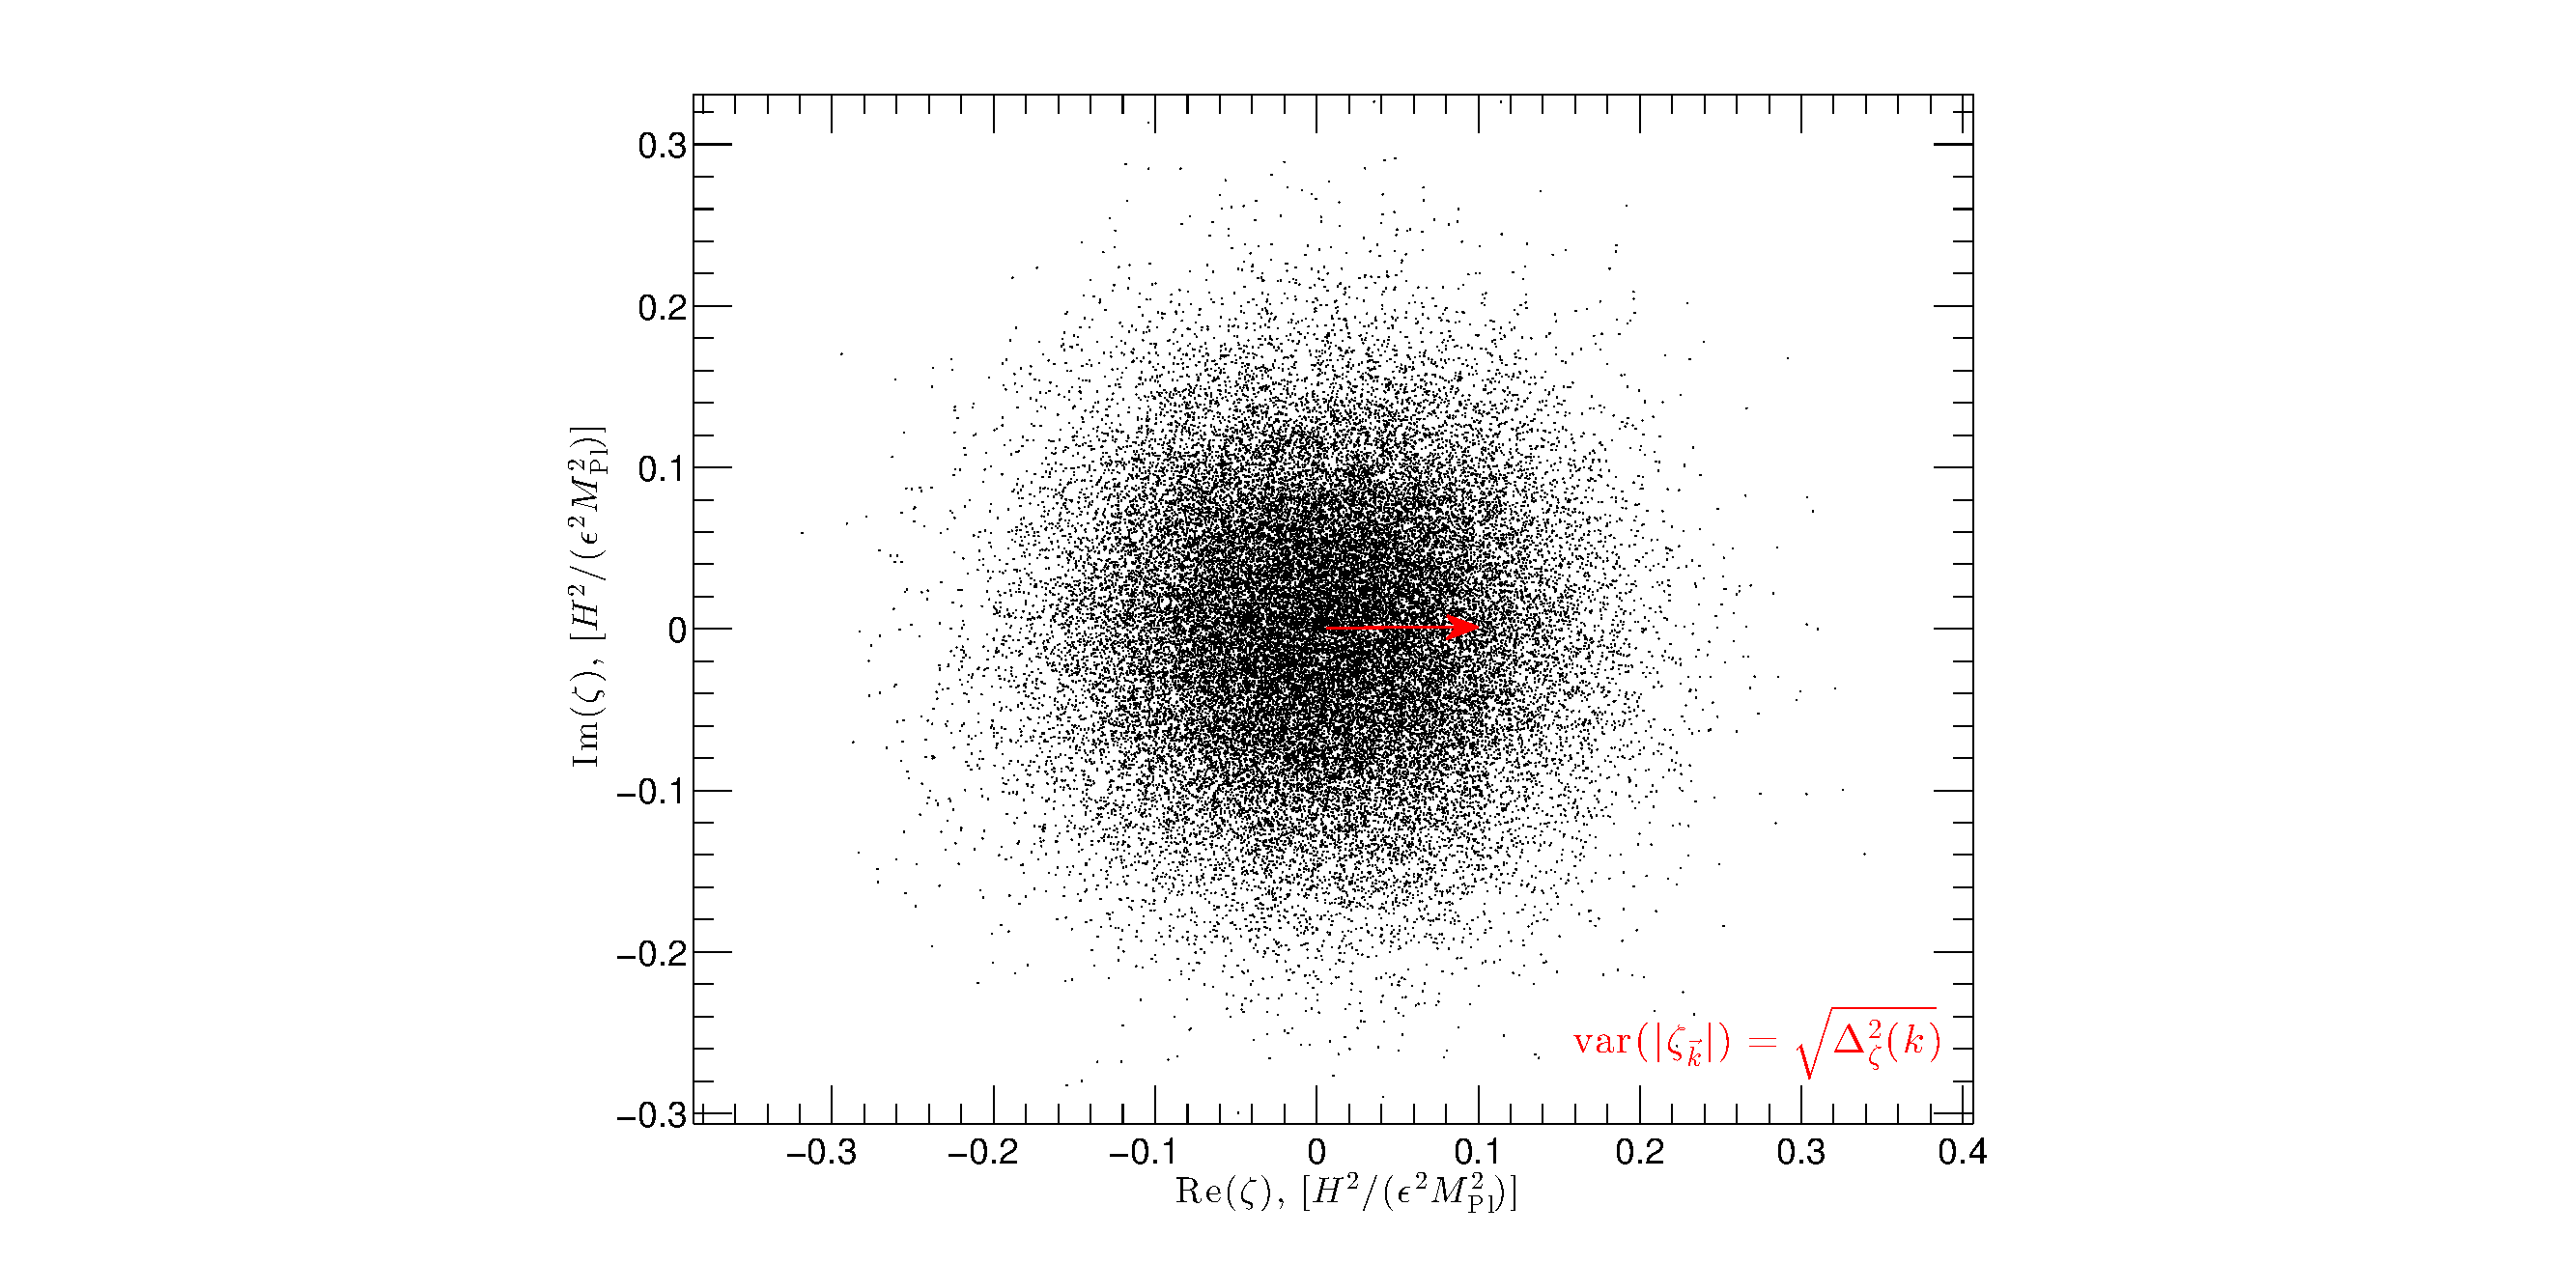
\includegraphics[trim = 80 -32 0 50 mm, width=.8\textwidth]{figures/onemodeThetadist.pdf}\\
\end{minipage}
\begin{minipage}[t]{0.48\linewidth}
\centering
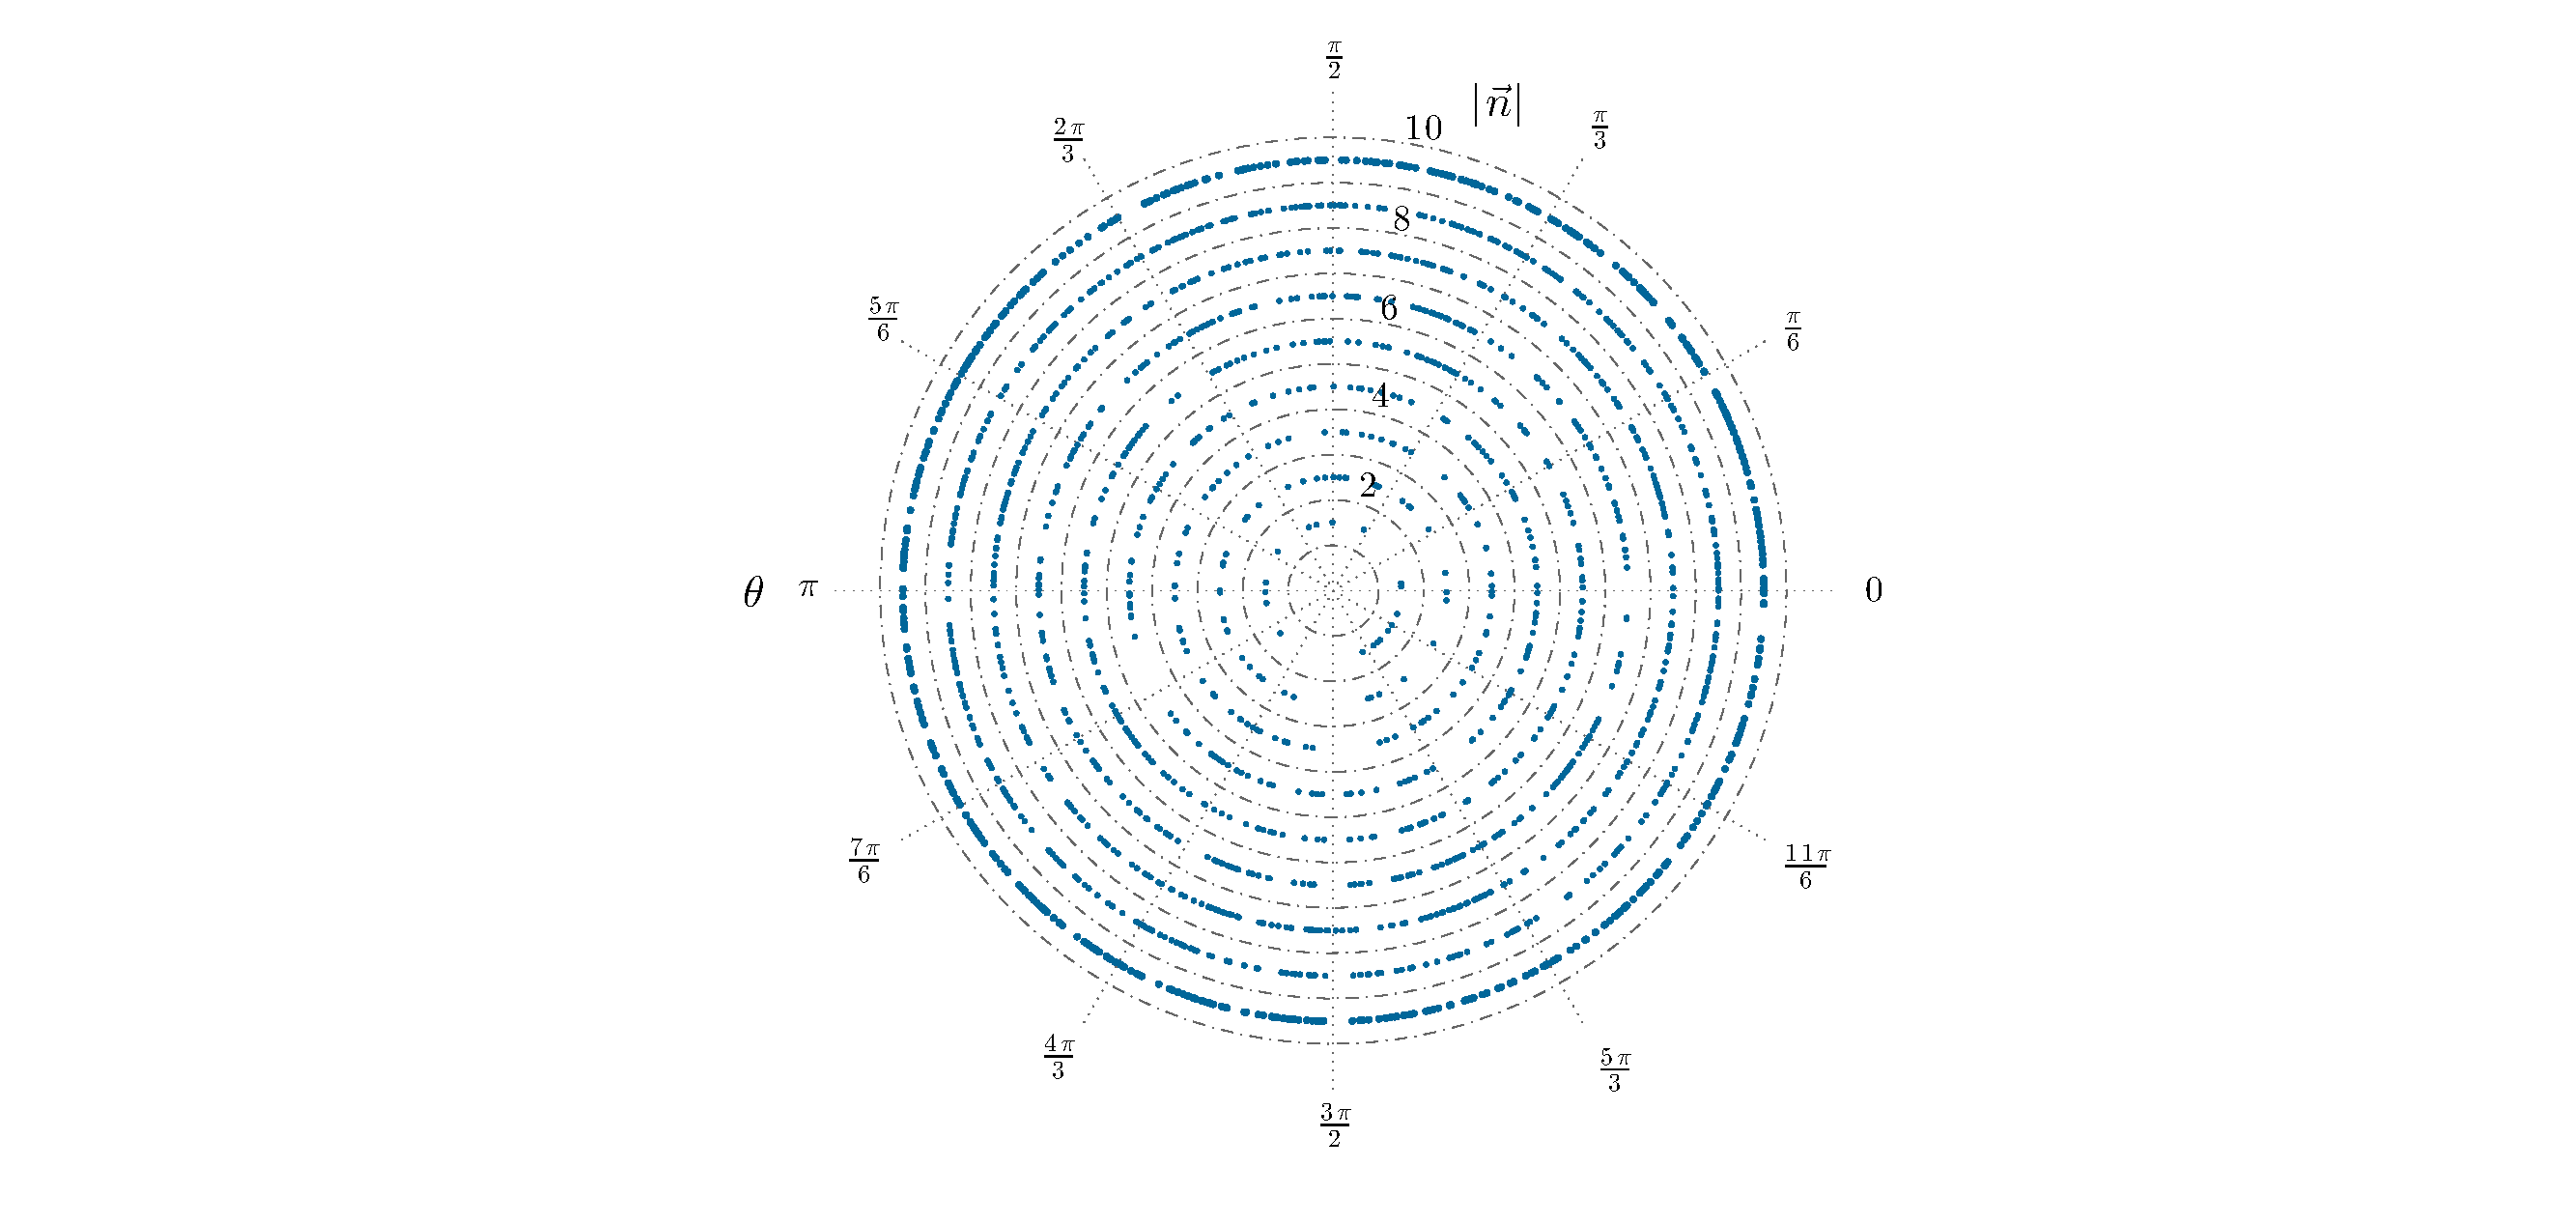
\includegraphics[trim = 0 0 0 0 mm, clip, width=.8\textwidth]{figures/first10modesThetadist.pdf}\\
\end{minipage}
\caption{\label{f:variations}
{\it Left panel}: \small{Distribution of the modes of $\zeta_{{\bf k}}$ at fixed $|{\bf k}|$.} {\it Right panel}: \small{Representation of  the norm of the first few $k$-modes ($|{\bf n}|$ from 2 to 10),
versus their random spatial angle $\theta$. If the individual modes were clustering around an angle, this would demonstrate that $\theta$ is actually not a uniformly distributed random variable, representing a serious challenge for inflation. Regardless of the distribution of $\theta$, observations of $\Delta_\zeta^2$ would not be affected. }
\vspace{-1cm}
}

\end{center}
\end{figure*}


One on the main uncertainties pertaining to inflation remains the shape of the potential for the scalar field $\varphi$, which determines the specific dynamics of inflation, e.g. its energy scale and the precise shape of the power spectrum, bi-spectrum, etc. it produces. Using our low-$k$ 3D reconstruction of the potential $\Phi$, it will also be possible to reconstruct the inflationary potential over a limited range of $\varphi$. This is achieved by expanding the potential locally around a fixed $\varphi=\varphi_*$ in a model independent way in terms of the ``slow-roll'' parameters. We can then define the inflationary vector parameter
\be
	\vec{\eta}=(H^2_*/\epsilon_*,\, \epsilon_*, \,\eta_*, \, (\eta_2)_*, \,(\eta_3)_*)\, ,
\ee
which defines uniquely a shape for the potential around $\varphi_*$. Here, the star quantities refer to their values when $\varphi=\varphi_*$. Using Bayes theorem, we then infer the probability of a given vector $\vec{\eta}$ given the data $a_y$, via the potential map $f_n$ (which we marginalize over), $\mathcal{P}(\vec{\eta}| a_{y})$,
\be
\mathcal{P}(\vec{\eta}| a_{y})=\frac{1}{(2\pi)^{p/2}} \left[\mathrm{Det}(C_{nn'})\mathrm{Det}(C_{yy'})\mathrm{Det}\,\mathbf{A}_{nn'}\right]^{-1/2}e^{\left\{\frac{1}{2}\mathbf{B}_{n}\mathbf{A}_{nn'}^{-1}\mathbf{B}_{n'}-\frac{1}{2}a^{\mathrm{T}}_{y'}C_{y'y}^{-1}a_{y} \right\}}\frac{\mathcal{P}(\vec{\eta})}{\mathcal{P}(a_{y})}\, ,
\ee
where $\mathcal{P}(\vec{\eta})$ is the prior on $\vec{\eta}$, ~$C_{n'n}^{-1}$ is a diagonal matrix with diagonal elements given by $1/|\zeta_{{\bf k}}|^2$, generalizing $1/{\sigma_{\bf n}^2}$ from our Gaussian prior
%\footnote{$C_{n'n}^{-1}$ therefore corresponds to the covariance matrix of the Gaussian prior for fixed $\vec{\eta}$ values}
and the $\mathbf{A}$ matrix and $\mathbf{B}$ vector are given by:
\be
	\mathbf{A}_{nn'}=\mathbf{R}_{ny'}C^{-1}_{y'y} \mathbf{R}_{yn'}+C_{nn'}^{-1}\, ,\qquad \qquad
	 \mathbf{B}_{n}=  \mathbf{R}_{ny'} C_{y'y}^{-1}  a_{y}\, .
\ee

\ni{\bf Detailed Approach Incorporating Planck Polarization Data:}
Up to this point, we have only considered the CMB temperature data. We anticipate making significant gains in map fidelity when we incorporate the Planck polarization data as well after it is made public. While these will be more sensitive to systematic effects (such as galactic dust and synchrotron emission), the additional signal to noise alone should allow us to make maps of higher spatial resolution. The prediction of E and B mode CMB polarization at low $\ell$ from a 3D model potential is more involved compared to the temperature field. Initial simple Monte Carlo ray tracing experiments suggest that this may be an instructive way to capture the dependence of the polarized radiation field on the underlying potential -- a challenge will be to capture this in a form that preserves our ability to use only the fast linear inversions described above.

%PJM: ROGER TO ADD FEW SENTENCES DETAIL ON PHYSICS BEING PROBED, AND RAY-TRACING EXPTS? I think this is enough

Then, we will carry out an extensive systematic error analysis, assessing sources of contamination from the various foregrounds (using the Planck products as templates) and quantifying the robustness of our results to them. We expect all our inferences to increase in precision as a result of including the polarization information; whether we can reach the commensurate degree of accuracy will depend on both the computational and modeling problems outlined here.

%PJM: SUFFICIENT ON SYSTEMATICS? WHAT OTHER GAINS/PITFALLS DO WE EXPECT? I think it better to say this is TBD

\ni{\bf Tree Representation and Non-Parametric Investigation of Gaussianity:}
There is another way to think about this problem. Let us build up the resolution of the potential on the CMB photosphere by increasing $\ell$ continuously from zero. Saddle points -- designated  S -- accompanied by extrema -- either maxima, designated H,  or minima, designated, L -- will be created. They will be accompanied by fresh separatrices -- the contours that pass through the saddles. These come in two types - ``lemniscates'', like an infinity symbol, and designated X, and ``lima\c cons'', with the shape of a pinched annulus, and designated K~\cite{Blandford:1986}. New separatrices may be created between existing separatrices or out of a contour encircling a $L$ or a $H$.  Occasionally, the inverse process -- annihilation -- will occur. If we designate the total number of maxima, minima, saddles, lemniscates and lima\c cons by $N_H,N_L,N_S,N_X,N_K$, respectively, then clearly $N_S=N_X+N_K=N_H+N_L-2$.\footnote{It is also instructive to calculate the Hessian matrix for the potential on the sphere and divide the sphere into ``H-zones'' (where both eigenvalues are negative), ``L-zones'' (where they are both positive) and ``S-zones'' (where they have opposite signs). These ``curvature maps''~\cite{Nye:1978} are complementary to the tree representation.}

The nesting of these contours defines a specific topology which suffices to describe all the equipotentials. It is convenient to represent it using a ``tree'' containing ``forks'' (corresponding to separatrices and labeled K or S ), and branches terminating on ``leaves'' (corresponding to extrema and labeled H or L)~\cite{west2001introduction}. There is only one ``path'' connecting any two leaves. Although our investigation has only begun, it is already clear that the statistics and structure of the tree, satisfy many rules if the underlying fluctuations are truly drawn from a random distribution, for example $N_K\sim N_X$ as $\ell\rightarrow\infty$. We propose to explore this novel approach to testing Gaussianity. We can actually extend this 2D approach on the photosphere to a 3D approach\footnote{Another generalization that we plan to explore is describe the topological arrangement of the polarization patterns~\cite{Scheuer:1977}.} exploring the nesting of the equipotential surfaces within the photosphere. This leads to similar type of tree. We propose to explore this as well with similar goals in mind.
\begin{figure}[t]
\centering
<<<<<<< HEAD
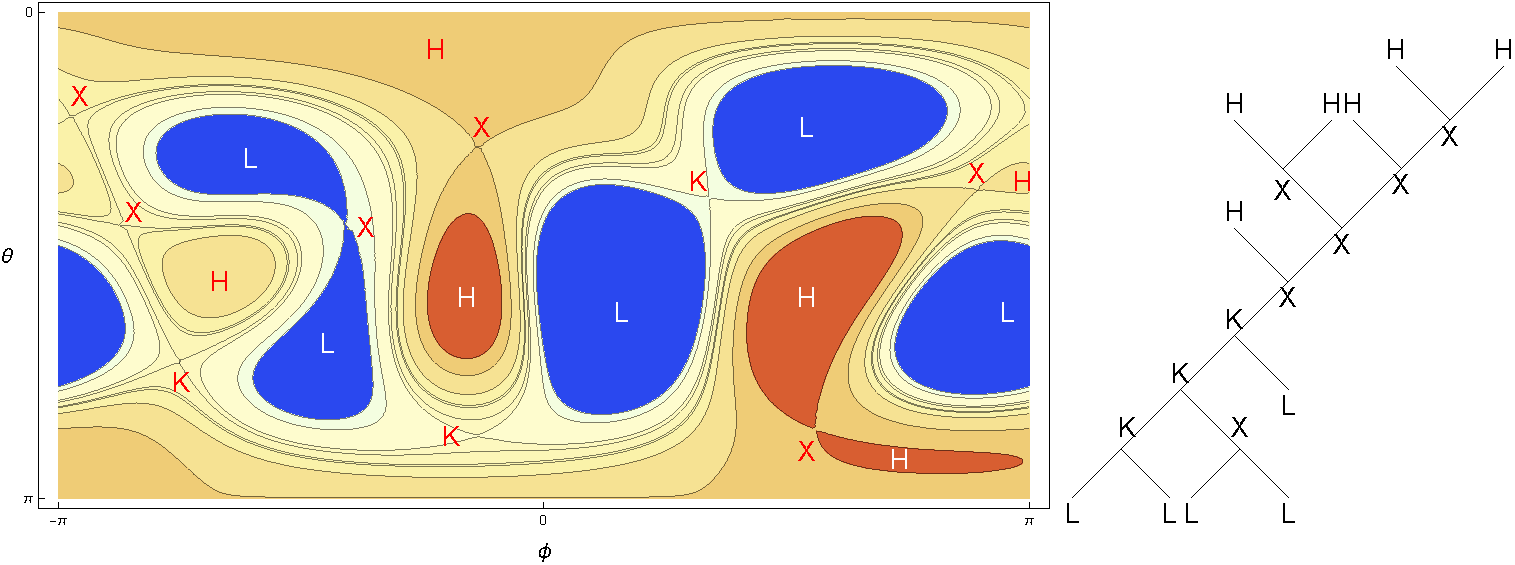
\includegraphics[width=6in]{figures/nsffig5.pdf}
\caption{{\small a) Nesting of separatrices for Planck data, with $\ell_{\rm max}=4.5$. The extrema, H, L and saddles, K, X are identified. b) Equivalent tree describing the same data.}}
=======
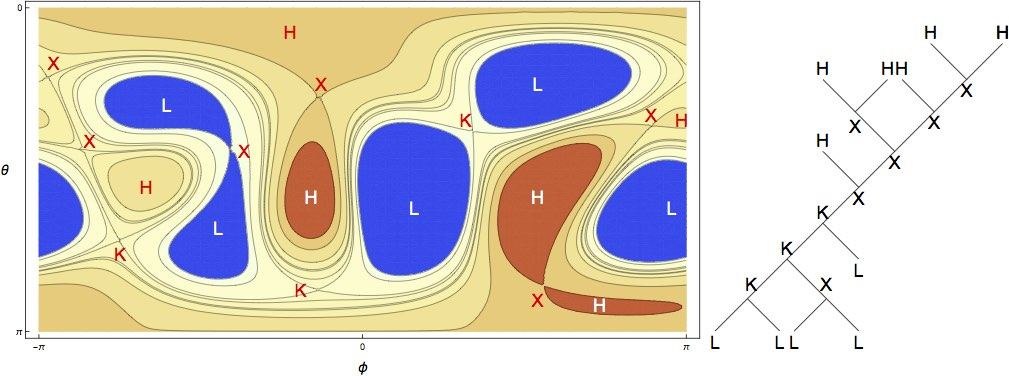
\includegraphics[width=0.9\linewidth]{figures/nsffig5.jpg}
\caption{{\small a) Nesting of separatrices for Planck data, with
$\ell_{\rm max}=4.5$. The extrema, H, L and saddles, K, X are
identified. b) Equivalent tree describing the same data.}}
>>>>>>> fff6f93c75898ae29f1264f24b6e5b58f9faaf30
\end{figure}


% - - - - - - - - - - - - - - - - - - - - - - - - - - - - - - - - - -

\subsection{Stage 2. From 3D to 4D: Incorporating Existing Volumetric Data}
\ni{\bf CMB Lensing and ISW Measurements:}
An important way to add 3D information is to include CMB lensing~\cite{Planck2015cosmopara}. A uniform CMB is unchanged by gravitational lensing. However, if there is a gradient in the background temperature, intervening structure will appear as extra power on the scale of intervening large scale structure.\footnote{More subtle manifestations including those involving polarization are possible~\cite{Hu:2002}, but this is the main effect.} The consequences are largest on much smaller scales than those in which we are primarily interested. However there are still integral effects with $\ell\sim30-100$ which are relevant. Furthermore the intense interest in the claim that inflationary B-modes have been detected~\cite{Planck2015cosmopara}  has focused much observational and analytical effort on this region of the spectrum. It is proposed to see if the addition of these measurements will improve the specification of the 3D body modes.

Similar remarks apply to the Integrated Sachs Wolfe effect which is caused by variation in the potential over time attributable to the cosmological constant at late times. It is proposed to see if such measurements can also contribute to the specification of structure on the largest scale, although here the challenge seems even greater.

\ni{\bf Galaxy Surveys and the Local Universe:}
Most of the use of surveys has been for drawing statistical inferences relating the growth of structure to the CMB emphasizing shorter length scales, notably those associated with BAO and the largest voids $\sim0.1$~Gpc. However, these same surveys can also be used to augment the long wavelength CMB data and improve the accuracy and resolution of the resulting 3D map. A good example is the SDSS/BOSS program,\footnote{http://www.sdss.org} which covered nearly a third of the sky with over a million redshifts and photometry on galaxies out to $z\sim0.7$.\footnote{21 cm redshift surveys provide an important complement to optical surveys but the survey volumes to date are comparatively modest.} For our purposes this translates to a comoving volume $\sim50{\rm Gpc}^3$, about 0.005 of the total. Surveys of much rarer quasars and the brightest star forming galaxies which extend to  $z\sim6$ provide much greater volumes over which the potential on Gpc scales can be estimated but with inferior precision.

It is helpful at this point to consider a volume limited-survey of objects out to some radius $r$. Suppose we have a set of objects, ($L^\ast$ galaxies, quasars, bright, star-forming galaxies $\dots$) with space density $n$ and we want to measure the amplitude of a given Fourier component with wave vector $k$ of the relative density perturbation associated with this potential $\delta\sim-2k^2\Phi/3a^2H^2$. Now the accuracy with which the amplitude of a single relative density perturbation Fourier mode can be measured is comparable with the precision with which the fractional density perturbation can be measured in a single region of size equal to the associated length scale. This is $\sim k^{3/2}n^{-1/2}$ and must exceed $\delta$. This suggests that the density of such objects must exceed $\sim H_0^4/c^2\Phi k_max$ if local surveys can possible connect with the CMB. A slightly more careful calculation indicates that making such a connection with existing survey and CMB data from stage 1 is just possible and so it is worth exploring this further. If this is achievable, then although the data increment will be small, its value will be much greater because it can act as a {\it phase reference} for anchoring the imperfectly specified modes measured by CMB observations.

\ni{\bf Constraints on Inflation:}
The newly developed effective field theory of large scale structure~\cite{Carrasco2012} has made great promises in terms of pushing constraints on the primordial Universe far beyond the scope of the CMB. This formalism relies on a separation of scales between the linear physics on large, cosmological scales in the infra-red (IR) and the non-linear physics on small scales in the ultra-violet (UV) (under $\sim10$ Mpc). These small scales are strongly coupled as a result of gravitational collapse. The UV modes are then integrated out in a way that yields a classical loop expansion correcting the dynamics of the linear IR theory. By pushing the theoretical control of modes with $k$ closer to the non-linear regime, a far greater amount of information becomes available. The future application of this method to current and upcoming surveys will certainly allow the improvement of our 3D map in accuracy and resolution, which will in turn be translated into better constraints on the inflaton potential, primordial non-Gaussianities, etc. Quantifying the astrophysical systematic errors will be an important part of this phase of the investigation: the connection between observed galaxy summaries such as their number density and the underlying potential will need to be quantified and explored. Both galaxy bias and halo bias will need to be incorporated into the treatment.

% - - - - - - - - - - - - - - - - - - - - - - - - - - - - - - - - - -

\subsection{Stage 3. Future Surveys}
Many facilities that are being planned or built will provide data relevant to our approach. In this phase of our program we will use simulated data for a selection of these future surveys to make forecasts of how our maps should improve, and look for new opportunities to exploit them.

\ni{\bf Ground-based CMB Telescopes:}
While there are exciting proposals for future space-based CMB measurements, most attention is currently focused on the next two generations -- Stages 3 and 4 -- of ground-based CMB telescopes, which have been proposed to deliver results in very roughly five and ten years respectively. While these are mostly focused on probing the physics of inflation and cosmological neutrinos \cite{CMBS4Inflation,CMBS4Neutrinos}, they will also improve the measurement of CMB temperature and E-mode polarization on the scales $\ell\lo200$ in which we are primarily interested, with signal to noise $\sim3\times10^{-4}$, roughly ten times higher than Planck.

\ni{\bf Survey Telescopes:}
Construction has begun on the Large Synoptic Survey Telescope (LSST\footnote{http://www.lsst.org/lsst/}), which will commence a decade-long survey in 2022. It will survey half the sky from Chile (with consequently very strong overlap with the ground-based CMB observations) in six optical and near infrared bands, detecting about ten billion galaxies out to $z\sim2$ for $L^\ast$ galaxies and $z\sim6$ for bright, star-forming galaxies and quasars \cite{LSSTOverviewPaper}. Its primary cosmological goal is to perform a multi-probe joint analysis (involving weak lensing, galaxy clustering, type Ia supernovae, time delay lenses and cluster number counts) to see if dark energy (and not just a cosmological constant) is responsible for cosmic acceleration \cite{LSSTDESCWhitePaper}. However, it  will, in practise, contribute to many more important cosmological tests. LSST will only provide photometric redshifts, but these will be well-calibrated by large spectroscopic surveys including that of DESI\footnote{http://desi.lbl.gov}, which is projected to measure $\sim20$ million redshifts to $z\sim1$ starting in 2018, and, potentially, the all-sky SphereX mission.\footnote{http://spherex.caltech.edu/} A complementary source of new local data will be the Euclid space mission\footnote{http://www.euclid-ec.org}, which is scheduled for a 2020 launch and which will carry out weak lensing, baryon acoustic oscillation and redshift space distortion measurements using 1.5 billion galaxies and 50 million redshifts over more than a third of the sky \cite{EuclidSciBook}. The proposed WFIRST-AFTA {http://wfirst.gsfc.nasa.gov} also has an impressive program in observational cosmology \cite{WFIRSTReport2015}, that will build on the LSST and Euclid surveys \cite{JainEtal2015}. Meanwhile, at radio wavelengths, the Canadian High Intensity Mapping Experiment (CHIME\footnote{http://chime.phas.ubc.ca}, see e.g.\ \cite{CHIME}) will measure BAO out to $z\sim2.5$ over half the sky.

As with the CMB, weak lensing and galaxy clustering observations can provide ``tomographic'' distance information and, in principle, should lead to a better map of the long wavelength potential perturbations. Systematic error control on these large scales is as yet uncharted territory: our 4D potential maps may have a role to play in this, effectively regularizing the local analysis on the largest angular scales. At the same time, local constraints on the 3D potential will pin down the  model considerably, improving our constraints on the inflation model.

\ni{\bf Epoch of Reionization:}
There is a large effort underway to probe the Epoch of Reionization, (EoR) $6\lo z\lo30$ through hydrogen line measurements. This is an exciting area of discovery, as the relevant physics depends upon many factors, notably first star formation and galaxy assembly that are very hard to anticipate.\footnote{JWST (http://www.jwst.nasa.gov), scheduled for launch in 2018, will also help indirectly in understanding the universe during this epoch but seems unlikely to provide quantitative measurements of very large scale structure.} The experiments will probe an ideal range of comoving radius $\sim8-12$~Gpc, interpolating between the CMB photosphere and local surveys,  for either contributing to or expanding upon our incorporating our 3D potential map.

On a longer time scale there are ambitious plans to construct an international Square Kilometer Array (SKA\footnote{https://www.skatelescope.org}). The long term goals include measuring the redshifts of a billion galaxies, performing weak lensing surveys and carrying out more sensitive surveys of the epoch of reionization (see  \cite{SKACosmology} and references therein). It is likely that the SKA capabilities and schedule will become better-defined over the lifetime of this proposed research program.

With a 4D potential model constrained both at $z=1100$ by the CMB and at $z=0.5$ by the Dark Energy surveys of the previous subsection, we will be able to make predictions about the large scale structure present in the volume at $6\lo z\lo30$ probed by EoR surveys. Such a prediction should assist in the interpretation of the survey data, and increase the fidelity of the measurements made there.

\subsection{Stage 4. Limits}
It is of interest to consider the limitations to what could be learned in principle about the idiosyncratic structure of our universe with {\it any} conceivable observing facility. Galaxy and quasar survey combined with EoR studies an CMB lensing should be able to give a detailed description of 4D potential though the resolution during the dark ages will be poor relative to that earlier and later epochs. Any explicit (not just statistical) linkage between large scale structure at recombination and today must strengthen investigations into basic physics questions including the presence of dynamical dark energy instead of a cosmological constant. Implicit in this approach is the opportunity to make statements about structure somewhat outside our horizon predicated on our adoption of the Gaussian prior on these large scales and involving the $\ell=0,1$ harmonics. This raises interesting issues of theoretical principle which we intend to try to clarify.

%%%%%%%%%%%%%%%%%%%%%%%%%%%%%%%%%%%%%%%%%%%%%%%%%%%%%%%%%%%%%%%%%%%%%%
%
%
% \begin{eqnarray}
% \Phi(x,\theta,\phi)&=&8\pi\sum_{\ell=0,2,\dots}^\infty(-1)^{\ell/2}\sum_{\bf k}^{\cal H}\Re[{\tilde\Phi}_{\bf k}]j_\ell(kx)\sum_{m=-\ell}^\ell Y_{\ell m}^\ast(\theta',0)Y_{\ell m}(\theta,0)\cos[m(\phi-\phi')]\cr
% &+&8\pi\sum_{\ell=1,3,\dots}^\infty(-1)^{(\ell+1)/2}\sum_{\bf k}^{\cal H}\Im[{\tilde\Phi}_{\bf k}]j_\ell(kx)\sum_{m=-\ell}^\ell Y_{\ell m}^\ast(\theta',0)Y_{\ell m}(\theta,0)\cos[m(\phi-\phi')].
% \end{eqnarray}
%
% where ${\bf k}=\pi[n_1,n_2,n_3]=k[\sin\theta'\cos\phi',\sin\theta'\sin\phi',\cos\theta']$, with $n_1,n_2,n_3$ integers and ${\bf x}=x[\sin\theta\cos\phi,\sin\theta\sin\phi,\cos\theta]$.  As $\Phi$ is real, we know that ${\tilde\Phi}_{\bf k}(-{\bf k})={\tilde\Phi}^\ast_{\bf k}({\bf k})$ and so we only need define the Fourier components over a hemisphere $\cal H$ in ${\bf k}$ space. We choose ${\cal H}=\{n_1>0\}\cup\{n_1=0,n_2>0\}\cup\{n_1=n_2=0,n_3>0\}$.
%
%
% \begin{eqnarray}
% \Phi(\bf x)&=&2\sum_{\bf k}^{\cal H}{\tilde\Phi}_{\bf k}\sum_{\ell=0}^\infty (2\ell+1)i^\ell P_\ell({\hat{\bf k}}\cdot{\hat{\bf x}})j_\ell(kx)\cr
% &=&8\pi\sum_{\bf k}^{\cal H}{\tilde\Phi}_{\bf k}\sum_{\ell=0}^\infty i^\ell j_\ell(kx)\sum_{m=-\ell}^\ell Y_{\ell m}^\ast(\theta',\phi')Y_{\ell m}(\theta,\phi)
% \end{eqnarray}
%
%  Let us start with the monopolar ($\ell=m=0$) term in Eq.~(3). For the moment, we just explore the partial potential associated with this single term, $\Phi^{00}({\bf x})=\sum{\tilde\Phi}^{00}_{\bf k}e^{i{\bf k}\cdot{\bf x}}$. We can expand this in terms of the original Fourier coefficients as ${\tilde\Phi}^{00}_{\bf k}=M^{00}_{\bf kk'}{\tilde\Phi}_{\bf k'}$, where $\bf k$, $\bf k'$ are shorthand for all the indices that specify individual spatial modes (summed when repeated) and we allow the matrix $M^{00}$ to pick out the real part of $\tilde\Phi_{\bf k}$. In this case,
% \begin{equation}
% M^{00}_{\bf kk'}=\frac14\int d{\bf x}{\rm sinc}kx\cos{\bf k'}\cdot{\bf x},
% \end{equation}
% which is best evaluated numerically. We proceed in this manner to evaluate all the necessary matrix elements $M^{\ell m}_{\bf kk'}$. (Of course there is an infinity of function spaces we could have chosen.)
%
% The strategy, then, is to start with a set of Fourier coefficients, $\tilde\Phi_{\bf k}$ which defines $\Phi({\bf x})$ within the box to sufficient resolution. We then use Eq.~(3) to define partial potentials associated with each spherical harmonic and sum them over $m$ to get a unique partial potential associated with each value of $\ell$. We then sum over all $\ell\le\ell_{\rm max}$ to give a low resolution version of the full potential which we designate as $\Phi(\ell_{\rm max},{\bf x})$. The benefit of this seemingly cumbersome procedure is that we do not have to include large values of $\bf k'$ for it to resemble an appropriately  smoothed version of the full potential and it accurately recovers the 2D potential as defined on the cosmic photosphere of radius $x_\gamma$. Conversely, as we increase $\ell_{\rm max}$, we converge quickly to the true potential at lower spatial resolution (Fig. ~1). An important point for what follows is that we can treat $\ell_{\rm max}$ not as an integer but as a continuous variable simply by adding a constant fraction in $\{0,1\}$  of all the $m$ components associated with $\ell=\ell_{\rm max}$.
%
% We now repeat this exercise for the equipotential surfaces within the sphere. The structurally stable stationary points in 3D are again highs (the Hessian has three negative eigenvalues), lows (three positive eigenvalues) and saddles (both signs). The separatrices are now surfaces passing through the saddles. Close to the saddles, they take the form of two cones with a common vertex on the saddle.
%
% What we must actually do first is to consider the equipotentials defined within the fundamental box with periodic boundary conditions so that opposite faces are identified. It is easy to see that the minimum number of stationary points in three dimensions is eight (six saddles a high and  a low). However, if we start with a sphere of sufficiently small radius, $x<1$ and $\ell=1$, there will be no stationary points within the sphere. We can then increase $x$ to unity bringing in additional stationary points. Next we increase $\ell$ as we did on the sphere. Provided that we consider the entire cube, each saddle is created with an accompanying $H$ or $L$.
